
% ---- begin preamble_alg.tex
\documentclass[11pt,a4paper]{article}
\usepackage[utf8]{inputenc}
\usepackage[T1]{fontenc}
\usepackage{mathpazo}
\usepackage[margin=2.5cm]{geometry}
\usepackage{amsmath,amssymb,amsthm,mathtools}
\usepackage{booktabs,enumitem,xcolor,array,needspace,caption}
\usepackage{placeins}
\usepackage[expansion=false]{microtype}
\usepackage{tikz,pgfplots}
\usetikzlibrary{arrows.meta,positioning,shapes.geometric,calc,fit,decorations.pathreplacing,backgrounds}
\pgfplotsset{compat=1.16}
\usepackage[most]{tcolorbox}
\usepackage[colorlinks=true,linkcolor=blue!45!black,citecolor=blue!45!black,urlcolor=blue!45!black]{hyperref}
\setlength{\parskip}{0.5em}\setlength{\parindent}{0pt}
\setlength{\emergencystretch}{2em}
\widowpenalty=10000 \clubpenalty=10000
\renewcommand{\arraystretch}{1.22}
\renewcommand{\topfraction}{0.9}\renewcommand{\bottomfraction}{0.8}\renewcommand{\textfraction}{0.1}\renewcommand{\floatpagefraction}{0.7}
\setlist{itemsep=2pt,topsep=3pt}
\newcolumntype{L}[1]{>{\raggedright\arraybackslash}p{#1}}

%---------- colours
\definecolor{cA}{HTML}{1F4E79}
\definecolor{cB}{HTML}{C0392B}
\definecolor{cC}{HTML}{1E8449}
\definecolor{cD}{HTML}{B9770E}
\definecolor{cG}{HTML}{7F8C8D}

%---------- theorem boxes
\makeatletter
\tcbset{labelfix/.style={before upper={\protected@edef\@currentlabel{\thetcbcounter}}}}% \ref now gives the theorem number, not the enclosing subsection number
\makeatother
\tcbset{thmstyle/.style={labelfix,enhanced,breakable,colback=cA!4,colframe=cA,boxrule=0.6pt,arc=1.5pt,
  left=6pt,right=6pt,top=4pt,bottom=4pt,fonttitle=\bfseries\sffamily\small,
  attach boxed title to top left={yshift=-2mm,xshift=4mm},boxed title style={colback=cA,arc=1pt,boxrule=0pt}}}
\newtcolorbox[auto counter,number within=section]{theorem}[2][]{thmstyle,title={Theorem~\thetcbcounter\ #2},#1}
\newtcolorbox[use counter from=theorem]{proposition}[2][]{thmstyle,title={Proposition~\thetcbcounter\ #2},#1}
\newtcolorbox[use counter from=theorem]{lemma}[2][]{thmstyle,title={Lemma~\thetcbcounter\ #2},#1}
\newtcolorbox[use counter from=theorem]{definition}[2][]{thmstyle,colback=cC!4,colframe=cC,boxed title style={colback=cC,arc=1pt,boxrule=0pt},title={Definition~\thetcbcounter\ #2},#1}
\newtcolorbox{intuition}[1][]{enhanced,breakable,colback=cD!6,colframe=cD,boxrule=0.5pt,arc=1.5pt,left=6pt,right=6pt,top=3pt,bottom=3pt,
  fonttitle=\bfseries\sffamily\small,title=Intuition,#1}
\newtcolorbox{caution}[1][]{enhanced,breakable,colback=cB!5,colframe=cB,boxrule=0.5pt,arc=1.5pt,left=6pt,right=6pt,top=3pt,bottom=3pt,
  fonttitle=\bfseries\sffamily\small,title=Warning,#1}
\theoremstyle{definition}
\newtheorem{example}{Example}[section]
\newtheorem*{remark}{Remark}
%---------- notation boxes and side notes (same visual vocabulary as the theorem boxes)
\newtcolorbox{notebox}[1]{enhanced,breakable,colback=cG!6,colframe=cG!75,boxrule=0.5pt,arc=1.5pt,left=8pt,right=8pt,top=5pt,bottom=4pt,
  fonttitle=\sffamily\bfseries\small,attach boxed title to top left={yshift=-2mm,xshift=4mm},boxed title style={colback=cG!75,arc=1pt,boxrule=0pt},before upper={\setlength{\parskip}{0.5em}},title={#1}}
\newtcolorbox{aside}[1]{enhanced,breakable,frame hidden,colback=cD!5,borderline west={1.8pt}{0pt}{cD},left=10pt,right=6pt,top=3pt,bottom=3pt,
  fontupper=\small,before upper={\setlength{\parskip}{0.55em}\textbf{\sffamily #1}\par\smallskip}}

%---------- status badges
\newcommand{\badge}[2]{\textcolor{#1}{\textsf{\footnotesize[#2]}}}
\newcommand{\proved}[1][]{\badge{cC}{proved#1}}
\newcommand{\modulo}[1]{\badge{cD}{proved mod.\ #1}}
\newcommand{\condl}{\badge{cD}{conditional}}
\newcommand{\openq}{\badge{cB}{open}}
\newcommand{\falsest}{\badge{cB}{false}}
\newcommand{\led}[1]{\textcolor{cG}{\textsf{\footnotesize(ledger #1)}}}
%---------- reading aids
\newtcolorbox{leadin}{enhanced,breakable,colback=white,colframe=cG,boxrule=0.5pt,arc=1pt,left=6pt,right=6pt,top=3pt,bottom=3pt,fontupper=\small,
  title={In this section},fonttitle=\sffamily\bfseries\small,coltitle=black,colbacktitle=cG!15}
\newcommand{\sectionbrief}[3]{\begin{leadin}\begin{description}[nosep,leftmargin=3.0cm,labelwidth=2.8cm]
  \item[Starting from] #1
  \item[Why this section] #2
  \item[Role in the paper] #3
  \end{description}\end{leadin}}

%---------- explained-edition boxes (added in this edition only)
\definecolor{cE}{HTML}{6C3483}
\newtcolorbox{explained}[1]{enhanced,breakable,colback=cE!4,colframe=cE,boxrule=0.6pt,arc=1.5pt,left=8pt,right=8pt,top=6pt,bottom=5pt,
  fontupper=\small,before upper={\setlength{\parskip}{0.45em}},
  fonttitle=\sffamily\bfseries\small,attach boxed title to top left={yshift=-2mm,xshift=4mm},boxed title style={colback=cE,arc=1pt,boxrule=0pt},title={Explained: #1}}
\newcommand{\edmark}[1]{\textsuperscript{\textcolor{cB}{\textsf{[#1]}}}}
\newtcolorbox{wstep}[1]{enhanced,colback=cA!3,colframe=cA!60,boxrule=0.5pt,arc=1pt,left=8pt,right=8pt,top=4pt,bottom=4pt,
  title={#1},fonttitle=\sffamily\bfseries\small,toptitle=1.5pt,bottomtitle=1.5pt}
\newcommand{\stepblock}[2]{\par\Needspace{6\baselineskip}\medskip\noindent\textbf{\sffamily Step #1: #2}\par\nopagebreak\smallskip}
\newtcolorbox{takeaway}{enhanced,breakable,frame hidden,colback=cA!3,borderline west={1.6pt}{0pt}{cA},left=8pt,top=2pt,bottom=2pt,fontupper=\small,before upper={\textbf{\sffamily Why it matters.}\ }}
\newtcolorbox{keypoint}{enhanced,breakable,frame hidden,colback=cC!5,borderline west={1.6pt}{0pt}{cC},left=8pt,top=2pt,bottom=2pt,fontupper=\small,before upper={\textbf{\sffamily Takeaway.}\ }}


%---------- macros
\newcommand{\R}{\mathbb{R}}\newcommand{\C}{\mathbb{C}}\newcommand{\N}{\mathbb{N}}\newcommand{\Z}{\mathbb{Z}}
\newcommand{\Ann}{\operatorname{Ann}}
\newcommand{\EP}{\mathrm{EP}}
\newcommand{\Eint}{E_{\mathrm{int}}}
\newcommand{\ring}{\mathcal{R}}
\newcommand{\Id}{\mathrm{Id}}
\newcommand{\Var}{V}
\newcommand{\dd}{\,\mathrm{d}}
\DeclareMathOperator{\Gcd}{gcd}
\DeclareMathOperator{\spn}{span}
\DeclareMathOperator{\dimc}{dim}

%---------- algorithm-edition additions: status badges and macros
\renewcommand{\proved}[1][]{\badge{cC}{implemented#1}}
\newcommand{\impl}{\badge{cC}{implemented, tested}}
\newcommand{\implu}{\badge{cD}{implemented, uncommitted}}
\newcommand{\proto}{\badge{cD}{prototype}}
\newcommand{\plan}{\badge{cB}{planned}}
\renewcommand{\openq}{\badge{cB}{open}}
\newcommand{\thy}[1]{\textcolor{cG}{\textsf{\footnotesize(theory #1)}}}
\newcommand{\bs}{\boldsymbol}
\DeclareMathOperator{\diag}{diag}
\DeclareMathOperator{\Cov}{Cov}
\DeclareMathOperator*{\argmin}{arg\,min}
\newcommand{\rhoR}{\rho}
\newcommand{\gN}{\gamma_N}
\newtcolorbox{symbols}{enhanced,breakable,colback=cG!4,colframe=cG,boxrule=0.5pt,arc=1.5pt,left=6pt,right=6pt,top=3pt,bottom=3pt,fontupper=\small,
  title={Symbols used here: what they are and where they come from},fonttitle=\sffamily\bfseries\small,coltitle=black,colbacktitle=cG!18}

% ---- end preamble_alg.tex


\title{\textbf{From Noisy Data to a Distribution over Equations}\\[4pt]
\large The algorithm behind the pipeline: spectral core, Bayesian layers, grouping and the loop\\[2pt]\normalsize\textit{Explained edition}}
\author{}
\date{October 2026}

\let\oldsection\section\renewcommand{\section}{\Needspace{9\baselineskip}\oldsection}
\let\oldsubsection\subsection\renewcommand{\subsection}{\Needspace{7\baselineskip}\oldsubsection}
\begin{document}
\maketitle

\begin{abstract}
\noindent
The analytic theory of the project says what a single exact solution of a linear constant-coefficient equation $P(\partial_t,\partial_x)u=0$ remembers about $P$: its factors, the components they generate, the interaction between terms. This document explains the \emph{algorithm} that turns that theory into a procedure working on \emph{noisy, scattered measurements}. Five layers are described. (i)~\emph{Interpolation}: a Gaussian-process posterior returns many plausible fields $\hat u_s$ with weights $\pi_s$. (ii)~\emph{Spectral core}, the only deterministic layer: on each $\hat u_s$ a Fourier transform in $x$ and a matrix pencil in $t$ produce points $(\lambda,i\kappa)$ of the dispersion variety, to which a \emph{structured} family of factors is fitted and compared by BIC. (iii)~\emph{Aggregation}: the factors of all samples form a weighted cloud, whose Dirichlet-process mixture gives a posterior on the number of factors. (iv)~\emph{Grouping}, which acts in mode space and on rectangles of the domain, never on raw data points. (v)~\emph{A Bayesian output layer}, built on the Friedrichs angle, giving credible intervals on the weights and the probability that the split exists. A sixth part, the \emph{loop} with its \emph{refinement on the raw data}, decides and labels the final answer; a long series of fixes made it robust (a section is devoted to them). A set of optional \emph{learned layers} (Phase~4) was built and evaluated, and mostly not adopted; it is told in the companion document. In the final benchmark the pipeline recovers the right factor set on all $30$ inputs without a false-confident answer. The text says, for each part, what is implemented and tested, what is prototype, what is only planned, and what the theory proves impossible.
\end{abstract}

\tableofcontents

\begin{notebox}{About this explained edition}
The structure follows the explained edition of the analytic paper. Every section opens with a box \emph{In this section} (starting point, reason, role). Theorems and algorithm statements sit in blue boxes; \textbf{purple ``Explained'' boxes} read the surrounding material step by step with small examples; orange boxes give intuition; red boxes are warnings. Status labels are \impl{} (code and tests exist), \implu{} (code exists, reported by its session, not yet committed), \proto{} (an experiment script only), \plan{}, and \openq{}. Grey tags such as \thy{T5} point to rows of the file \texttt{analysis/THEORY\_TO\_ALGO.md}, which links each algorithmic choice to a result of the analytic work; Appendix~\ref{app:tags} states each tagged result in one sentence. A new symbol is always explained where it first appears, and each section opens with a box ``Symbols used here: what they are and where they come from.''
\end{notebox}
\bigskip


% ---- begin s01_intro.tex
\section{Introduction}\label{sec:intro}
\sectionbrief
{noisy measurements $(t_i,x_i,y_i)$ with $y_i\approx u(t_i,x_i)$ of a field that solves an unknown linear constant-coefficient equation in one time and one space variable; the analytic theory (identification, factor decomposition, interaction term) is taken as given.}
{to turn exact theorems into a procedure whose input is imperfect data, and to say exactly where the exactness is lost.}
{this section frames the three tasks, shows the whole pipeline in one figure and lists what each stage relies on. Sections~\ref{sec:interp}--\ref{sec:loop} then describe the stages one by one.}

\subsection{The question}
Throughout, $u(t,x)$ is a field (a function of time $t$ and one space coordinate $x$) known on a rectangle $\Omega$ of the $(t,x)$-plane, and $P(\partial_t,\partial_x)u=0$ is the linear constant-coefficient equation it solves, with $P$ unknown; all the symbols are introduced in Section~\ref{sec:prelim}. The analytic work answers three questions for an exact solution $u$: which operator $P$ does $u$ determine (Q1), how does $u$ split into the components generated by the factors of $P$ (Q2), and what part of $u$ is due to no single term but to their interplay (Q3). Here the data are finitely many noisy samples, so the answers must change form:
\begin{enumerate}[label=\textbf{A\arabic*.},leftmargin=1.1cm,nosep]
\item \textbf{Which factors, with which coefficients, and how sure are we?} The output is a \emph{probability distribution over factor structures}, never a single ``identified'' law.
\item \textbf{How much of the signal does each factor carry?} Weights $w_j$ with credible intervals that widen when the components are hard to separate.
\item \textbf{Are the factors really separate or tangled?} The numbers $\gamma_N$, $c_F$ and the interaction ratio $\rho$, as distributions over interpolants.
\end{enumerate}
The setting is no longer purely analytic: part of the algorithm is statistical. The design rule is that the delicate analytic part stays deterministic and is called as a black box, and everything around it is Bayesian.

\subsection{The pipeline}
\begin{figure}[!htb]
\centering
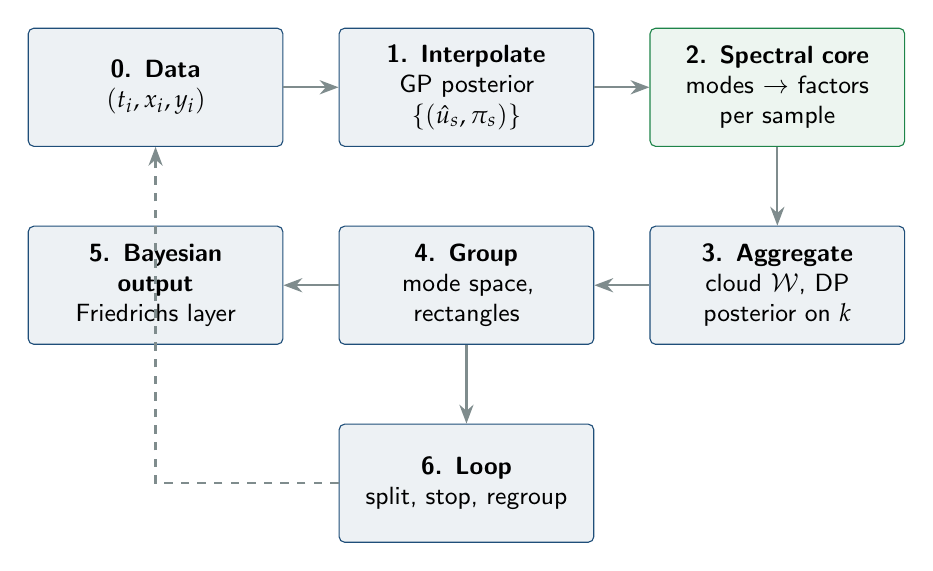
\begin{tikzpicture}[node distance=7mm,
  det/.style={draw=cC,fill=cC!8,rounded corners=2pt,minimum height=15mm,text width=3.0cm,align=center,font=\small\sffamily},
  stat/.style={draw=cA,fill=cA!8,rounded corners=2pt,minimum height=15mm,text width=3.0cm,align=center,font=\small\sffamily},
  arr/.style={-{Stealth[length=2.4mm]},thick,cG}]
\node[stat] (d) {\textbf{0. Data}\\ $(t_i,x_i,y_i)$};
\node[stat,right=of d] (i) {\textbf{1. Interpolate}\\ GP posterior\\ $\{(\hat u_s,\pi_s)\}$};
\node[det,right=of i] (c) {\textbf{2. Spectral core}\\ modes $\to$ factors\\ per sample};
\node[stat,below=10mm of c] (a) {\textbf{3. Aggregate}\\ cloud $\mathcal W$, DP\\ posterior on $k$};
\node[stat,left=of a] (g) {\textbf{4. Group}\\ mode space,\\ rectangles};
\node[stat,left=of g] (b) {\textbf{5. Bayesian\\ output}\\ Friedrichs layer};
\node[stat,below=10mm of g] (l) {\textbf{6. Loop}\\ split, stop, regroup};
\draw[arr] (d)--(i); \draw[arr] (i)--(c); \draw[arr] (c)--(a); \draw[arr] (a)--(g); \draw[arr] (g)--(b);
\draw[arr] (g)--(l); \draw[arr,dashed] (l.west) -| ($(d.south)+(0,-4mm)$) -- (d.south);
\end{tikzpicture}
\caption{The pipeline. Only the green box is deterministic. The dashed arrow is the recursion: each group becomes a new data set.}\label{fig:pipeline}
\end{figure}

\begin{table}[!htb]
\centering\small
\begin{tabular}{@{}L{2.6cm}L{5.6cm}L{3.2cm}L{2.6cm}@{}}
\toprule
Stage & What it does & Relies on & Status\\\midrule
1 Interpolation & GP posterior on a grid from scattered data; hyperparameters marginalised & \thy{T11}, \thy{T12} & \impl{}; band coverage within $\pm5$ points in $11$ of $12$ cells\\
2 Spectral core & FFT in $x$, matrix pencil in $t$; structured factor fit, BIC over 85 structures; components, weights, $\gamma_N$; per-bin correlated noise & \thy{T1}, \thy{T2}, \thy{T5}, \thy{T15} & \impl{}\\
3 Aggregation & weighted cloud of factor coefficients; DP mixture; $k_{\mathrm{eff}}$ & \thy{T12} & \impl{}\\
4 Grouping & mode space, rectangles with quadtree & \thy{T1}, \thy{T5}, \thy{T8} & \impl{}\\
5 Bayesian output & posterior on components, $P(\text{split})$, intervals following $\theta_F$; raw-data evidence & \thy{T5}, \thy{T6} & \impl{}; coverage logged $0.85$--$1.00$, not certified\\
6 Loop & degree growth with a held-out guard, regroup at fixed $k$, recursion per factor, refinement on the observations & \thy{T15} & \impl{}; thresholds still hand defaults\\
6b Refinement and decision & raw-data evidence, support path, exact splits, goodness-of-fit downgrades, intervals (Sec.~\ref{sec:refine}) & \thy{T17}, T44--T103 & \impl{}; final benchmark $30/30$ right\\
7 Learned layers & seeds for the exponential fit, calibration, failure validator, remedy table (Phase~4; see the companion document) & \thy{T10} & evaluated; none ships except an exact memo; pipeline $=$ pipeline $+$ ML\\
\bottomrule
\end{tabular}
\caption{The stages, the theory each one rests on, and their present status.}\label{tab:stages}
\end{table}

\subsection{Notation at a glance}
Every symbol is introduced in Section~\ref{sec:prelim} or in the box that opens the section that needs it; this table only collects the main ones and says where each comes from.
\begin{table}[!htb]
\centering\small
\begin{tabular}{@{}L{2.9cm}L{7.0cm}L{3.0cm}@{}}
\toprule
Symbol & Meaning & Comes from\\\midrule
$u(t,x),\ \Omega$ & the field, and the rectangle of the $(t,x)$-plane where it is known & the data; Sec.~\ref{sec:prelim}\\
$P,\ Q_j$ & the unknown operator (as a polynomial in $\tau,\xi$) and its factors & the theory; Sec.~\ref{sec:prelim}\\
$\kappa,\ \lambda$ & wavenumber (spatial frequency, real) and rate of evolution in time (complex) of a mode $e^{\lambda t+i\kappa x}$ & Sec.~\ref{sec:prelim}\\
$m_j,\ dx_j,\ \mathcal M$ & degree in $\tau$ and bound on the degree in $\xi$ of factor $j$; a \emph{structure}, the list of these shapes (85 candidates) & Sec.~\ref{sec:prelim}; the algorithm\\
$\hat u_s,\ \pi_s,\ N_s$ & the $s$-th posterior field, its weight, the number of fields & Sec.~\ref{sec:interp}\\
$\sigma_\lambda$ & uncertainty of a mode's rate $\lambda$ (Cram\'er--Rao) & Sec.~\ref{sec:core}\\
$u_j,\ w_j$ & component of factor $j$; its weight $\|u_j\|/\sum_k\|u_k\|$ & Sec.~\ref{sec:core}\\
$\gamma_N,\ c_F$ & how well the components can be separated; $\gamma_2=1-c_F$ & theory; Sec.~\ref{sec:core}\\
$\rho$ & interaction ratio $\|\Eint\|/\|u(T)-u_0\|$ of an evolution factor & theory; Sec.~\ref{sec:core}\\
$\bs\beta^{(s)}_j$ & coefficient vector of factor $j$ in sample $s$ & Sec.~\ref{sec:agg}\\
$\mathcal W$ & the weighted cloud of all the $\bs\beta^{(s)}_j$ & Sec.~\ref{sec:agg}\\
$k_{\mathrm{eff}}$ & $\exp(-\sum_jW_j\log W_j)$, effective number of factors & Sec.~\ref{sec:agg}\\
\bottomrule
\end{tabular}
\caption{Notation guide.}
\end{table}

\subsection{Roadmap}
Section~\ref{sec:prelim} recalls why exponentials are the right ``basis''. Section~\ref{sec:interp} is stage 1, Section~\ref{sec:core} stage 2 (the longest), Section~\ref{sec:agg} stage 3, Section~\ref{sec:group} stage 4, Section~\ref{sec:bayes} stage 5 and Section~\ref{sec:loop} the loop. Section~\ref{sec:q} answers the two design questions put to the machine-learning side, Section~\ref{sec:train} describes the trainable version, Section~\ref{sec:example} follows one example from data to output, and Section~\ref{sec:limits} lists the limits.

% ---- end s01_intro.tex


% ---- begin s02_prelim.tex
\section{Notation from scratch: symbols, exponentials, the dispersion variety}\label{sec:prelim}
\sectionbrief
{nothing beyond calculus: a function $u(t,x)$ of time and one space variable, and derivatives. Every symbol used later is introduced here, in the order in which it is needed, with the reason it exists.}
{the algorithm works on exponential modes, not on a chosen dictionary of functions. To follow it one must know what a symbol, a factor, a wavenumber and a mode are; this section builds them one at a time.}
{foundation for everything after it. Each later section begins with a box listing the symbols it uses and where each comes from.}

\subsection{The objects: field, region, equation}
\begin{symbols}
\begin{tabular}{@{}L{2.3cm}L{6.2cm}L{4.5cm}@{}}
$t,\ x$ & time and one space coordinate (a rod, a string, a line) & the physical setting\\
$\Omega$ & the region of the $(t,x)$-plane where the field is known, a rectangle $[t_0,t_1]\times[x_0,x_1]$ here & the data\\
$u(t,x)$ & the \emph{field}: a number (real or complex) at each point of $\Omega$ (a temperature, a displacement) & the data, up to noise\\
$\partial_t,\ \partial_x$ & partial derivatives $\partial/\partial t$ and $\partial/\partial x$ & calculus\\
$P(\partial_t,\partial_x)$ & a \emph{linear operator with constant coefficients}: a polynomial in the derivatives, e.g.\ $\partial_t-D\partial_x^2$ (heat); the equation is $Pu=0$ & the unknown of the problem\\
\end{tabular}
\end{symbols}

The problem is: given measurements of $u$ on $\Omega$, find $P$. ``Linear with constant coefficients'' means $P$ is a sum of terms $c\,\partial_t^a\partial_x^b$ with numbers $c$ (not functions of $t$ or $x$), so that for example $\partial_t u+\partial_xu=0$ (transport at speed $1$) and $\partial_tu-D\,\partial_x^2u=0$ (heat, with diffusion constant $D>0$) belong to the class, while $\partial_tu+u\,\partial_xu=0$ (Burgers) does not.

\subsection{Derivatives become polynomials: the symbol}
Because the coefficients are constant, an operator is \emph{multiplication-like}: composing $\partial_t^a\partial_x^b$ with $\partial_t^{a'}\partial_x^{b'}$ simply adds exponents, exactly as in a ring of polynomials. So one introduces two formal variables, $\tau$ standing for $\partial_t$ and $\xi$ standing for $\partial_x$, and writes the operator as a polynomial $P(\tau,\xi)$, its \emph{symbol}. Example: $\partial_t-D\partial_x^2\ \leftrightarrow\ \tau-D\xi^2$. The reason for the change of notation is that polynomials can be \emph{factored}, and factoring is the central operation of the method: if $P(\tau,\xi)=Q_1(\tau,\xi)\,Q_2(\tau,\xi)$ then the operator is the composition of the two simpler operators $Q_1(\partial)$ and $Q_2(\partial)$. The $Q_j$ are called the \emph{factors} (they are the ``basic behaviours'' of the equation: transport, diffusion, \dots).

\subsection{An exponential is an eigenfunction}
For a field of the form $e^{\lambda t+\mu x}$ (where $\lambda,\mu$ are complex numbers) every derivative just multiplies by a number: $\partial_te^{\lambda t+\mu x}=\lambda e^{\lambda t+\mu x}$ and $\partial_xe^{\lambda t+\mu x}=\mu\, e^{\lambda t+\mu x}$. Therefore
\begin{equation}\label{eq:eigen}
P(\partial_t,\partial_x)\,e^{\lambda t+\mu x}=P(\lambda,\mu)\,e^{\lambda t+\mu x}.
\end{equation}
So $e^{\lambda t+\mu x}$ is a solution of $Pu=0$ exactly when $P(\lambda,\mu)=0$. The set $V(P)=\{(\lambda,\mu)\in\C^2:\ P(\lambda,\mu)=0\}$ is the \emph{dispersion variety} (a curve in the plane of the two numbers); the word ``dispersion'' comes from physics, where $\lambda$ as a function of the spatial frequency is called the dispersion relation.

\subsection{The wavenumber $\kappa$ and the rate $\lambda$}
On a bounded region one expands in spatial exponentials that stay bounded in $x$, so $\mu$ is taken purely imaginary, $\mu=i\kappa$ with $\kappa$ \emph{real}. The two numbers then have clear roles:
\begin{itemize}[nosep]
\item $\kappa\in\R$, the \emph{wavenumber} (Fourier variable conjugate to $x$): which spatial exponential $e^{i\kappa x}$ we look at; its spatial period is $2\pi/|\kappa|$;
\item $\lambda\in\C$, the \emph{rate}: how the equation makes that exponential evolve in time; $\operatorname{Re}\lambda<0$ means decay, $\operatorname{Im}\lambda\neq0$ means oscillation or motion.
\end{itemize}
A pair $(\kappa,\lambda)$ with $P(\lambda,i\kappa)=0$ is a \emph{mode}: the function $e^{\lambda t+i\kappa x}$ is an exact solution. Substituting $\mu=i\kappa$ in the symbol means $\xi=i\kappa$.

\begin{notebox}{What $\kappa$ is (and what it is not)}
$\kappa$ is the \emph{Fourier variable} conjugate to $x$: the frequency of the exponential $e^{i\kappa x}$ in which a field is expanded. It is called a ``wavenumber'' only by convention, and it has \emph{nothing to do with the wave equation}: it appears identically for transport, heat, beam, Schr\"odinger and so on. (If one wants a length, $2\pi/|\kappa|$ is the spatial period of that exponential.) The exponentials $e^{\lambda t+i\kappa x}$ are the ``basis functions'' of the method: $\kappa$ labels which basis function, and $\lambda$ is the rate at which the equation makes it evolve in time. The wave equation is just one of ten test cases.
\end{notebox}

\subsection{The Fourier transform in $x$ and the amplitudes}
Because a general field is a superposition of modes, one separates them by the Fourier transform in $x$,
\[
\hat u(t,\kappa)=\int u(t,x)\,e^{-i\kappa x}\dd x\qquad(\text{on a grid: the discrete FFT}).
\]
If $u=\sum_mA_m\,e^{\lambda_mt+i\kappa_mx}$, then $\hat u(t,\kappa)$ keeps, at the frequency $\kappa$, only the modes with $\kappa_m=\kappa$: $\hat u(t,\kappa)=\sum_{m:\kappa_m=\kappa}A_me^{\lambda_mt}$. The numbers $A_m\in\C$ are the \emph{amplitudes} (how much of each mode is present). Extracting the $\lambda_m$ and $A_m$ from the time series $\hat u(\cdot,\kappa)$ is the job of Section~\ref{sec:modes}.

\begin{explained}{from an equation to a curve of points}
\textbf{Step 1: transport.} $u_t+u_x=0$ has symbol $\tau+\xi$. A mode $e^{\lambda t+i\kappa x}$ is a solution iff $\lambda+i\kappa=0$, i.e.\ $\lambda=-i\kappa$. In the $(\kappa,\lambda)$ plane the modes lie on a straight line: a bump $g(x-t)=\int\hat g(\kappa)e^{i\kappa(x-t)}\dd\kappa$ is a sum of modes with $\lambda=-i\kappa$.

\medskip\textbf{Step 2: heat.} $u_t=Du_{xx}$ has symbol $\tau-D\xi^2$, so $\lambda=D(i\kappa)^2=-D\kappa^2$: a parabola, real and negative (every mode decays).

\medskip\textbf{Step 3: wave.} $u_{tt}=c^2u_{xx}$ has symbol $\tau^2-c^2\xi^2$, so $\lambda=\pm ic\kappa$: two lines through the origin. At $\kappa=0$ the two roots coincide: this is the shared mode responsible for the ambiguity $\delta(P)=1$ of the theory (explained in Section~\ref{sec:core}).

\medskip\textbf{Step 4: the algorithm reads the curve, not the function.} A solution of $P=(\tau+\xi)(\tau-D\xi^2)$ (transport plus a diffusing wave) produces, at each $\kappa$, \emph{two} rates: $-i\kappa$ and $-D\kappa^2$. The set of all measured $(\kappa,\lambda)$ sits on the union of a line and a parabola. Finding the factors of $P$ means finding the curves on which the points lie: this is a geometric fitting problem, which is the content of Section~\ref{sec:core}.
\end{explained}

\subsection{Why exponentials are the right ``basis''}
The Ehrenpreis--Palamodov principle (a theorem of the analytic theory, \thy{T25}) says that on a convex region every solution of $Pu=0$ is a superposition (an integral) of such exponentials over $V(P)$. So in this class the exponentials are universal: no dictionary of functions has to be chosen. This is the reason the first design question (Section~\ref{sec:q}) has a clean answer.

\subsection{Monic symbols, degrees, and structures}
\begin{symbols}
\begin{tabular}{@{}L{2.3cm}L{6.2cm}L{4.5cm}@{}}
$Q(\tau,\xi)$ & one factor of the symbol & factorisation of $P$\\
$m$ & degree of $Q$ in $\tau$ (``order in time''): $m=1$ for transport, heat; $m=2$ for wave, beam & the factor itself\\
$p_k(\xi)$ & coefficients of $Q$ as a polynomial in $\tau$; each is a polynomial in $\xi$ & the factor itself\\
$dx$ & upper bound for the degrees of the $p_k$ in $\xi$ (``order in space''); a \emph{bound}, not the true degree & chosen by the algorithm\\
structure $\mathcal M$ & the list $((m_1,dx_1),\dots,(m_k,dx_k))$ of shapes of the factors & chosen by the algorithm\\
\end{tabular}
\end{symbols}
The code fixes the shape of a factor to be \emph{monic in $\tau$}, meaning that its leading coefficient in $\tau$ is $1$:
\begin{equation}\label{eq:monic}
Q(\tau,\xi)=\tau^m+\sum_{k<m}p_k(\xi)\,\tau^k,\qquad \deg p_k\le dx .
\end{equation}
Monic in $\tau$ is the setting in which the identification theorems apply \thy{T13}: the evolution in time determines everything (one can solve for $\partial_t^mu$). For example $\tau-a_1\xi$ is a factor with $m=1$, $dx=1$ (transport, speed $-a_1$), $\tau-a_2\xi^2$ has $m=1$, $dx=2$ (diffusion), and $\tau^2-c^2\xi^2$ has $m=2$, $dx=2$. A \emph{structure} is then a hypothesis about the shapes of all factors, for example $((1,1),(1,2))$ for ``one factor $\tau-a_1\xi$ times one factor $\tau-a_2\xi^2$'' (transport times diffusion), whose unknowns are $a_1,a_2$ and, more generally, all the coefficients allowed by the bounds $dx_j$.

\begin{explained}{a reader asks: exponentials, but exponential polynomials cause ambiguity?}
Two different things are easily confused here.

\medskip\textbf{Step 1: what is ambiguous.} If two factors share a root, a solution may contain $t\,e^{\lambda t}$ (a polynomial times an exponential), and a mode $e^{\lambda t+i\kappa x}$ lying on two factors' curves can be assigned to either one. The \emph{ambiguity} $\delta(P)$ is therefore about \emph{which factor owns a mode}, not about the representation of the field.

\medskip\textbf{Step 2: why exponentials stay the basis.} Every solution is still a superposition of exponentials, with polynomial prefactors only at repeated roots; these are exceptional points (for the wave, only $\kappa=0$). The representation is complete. Changing to another basis would not remove the ambiguity: it lives in the solution space, not in the choice of functions.

\medskip\textbf{Step 3: what the algorithm does about it.} Exponential-polynomial data never identify the annihilator itself, only a law \emph{relative to a class} \thy{T13}. So (i) a confluent test $(A+Bt)e^{\lambda t}$ labels such cases \texttt{UNDECIDED} rather than guessing (Section~\ref{sec:confluent}); (ii) a shared mode is split equally, the minimum-norm representative (Section~\ref{sec:core}); (iii) the output never says ``identified''. Exponentials are the right language; the ambiguity is reported, not hidden.
\end{explained}

\begin{takeaway}
The unknowns are the coefficients of the polynomials $p_k$. A mode $(\kappa,\lambda)$ is a measurement of the variety: each one gives one equation $Q(\lambda,i\kappa)=0$ on these coefficients. This is why the first design question has a clean answer inside the linear constant-coefficient class and a hard one outside it (Section~\ref{sec:q}).
\end{takeaway}

% ---- end s02_prelim.tex


% ---- begin s03_interp.tex
\section{Stage 1: interpolation with probabilities}\label{sec:interp}
\sectionbrief
{scattered noisy samples $(t_i,x_i,y_i)$, possibly periodic in $x$, no knowledge of the equation.}
{the analytic core needs a field on a regular grid, and because data are finite there is no single correct field. The stage must return \emph{many} fields with weights, not one.}
{first link of the chain. Its output $\{(\hat u_s,\pi_s)\}$ is what the core is run on, sample by sample.}

\begin{symbols}
\begin{tabular}{@{}L{2.5cm}L{6.0cm}L{4.4cm}@{}}
$(t_i,x_i,y_i)$, $i\le n$ & the $n$ measurements: place $(t_i,x_i)$ and measured value $y_i\approx u(t_i,x_i)$ & the data\\
$\varepsilon_i,\ s_n$ & measurement noise (random error) and its standard deviation & assumed Gaussian\\
$f$ & the unknown smooth function we fit; it equals the field $u$ up to the constant $c$ & the quantity inferred\\
$c$ & constant offset (mean level) of the standardised data & preprocessing\\
kernel $k(\cdot,\cdot)$ & a function giving the prior covariance of $f$ between two points: it encodes how smooth $f$ is & the choice of model\\
$k_t^{(r)},k_x^{(r)}$, $R$ & factors of the kernel in $t$ and in $x$ for the $r$-th of $R$ summed terms (``separable'' = a product of a function of $t$ and one of $x$) & the choice of model\\
$s_r,\ \ell_t^r,\ \ell_x^r$ & amplitude of term $r$ and its correlation lengths in $t$ and in $x$ (the distance over which $f$ stays correlated) & hyperparameters\\
$\eta$ & the list of all hyperparameters $(s_r,\ell_t^r,\ell_x^r,s_n,c)$, in logarithms & unknown, marginalised\\
$\bar f,\ K_{\mathrm{post}}$ & posterior mean and covariance of $f$ given the data & output of the GP\\
$N_s$ samples, $\hat u_s$, $\pi_s$ & $N_s$ fields drawn from the posterior on a regular grid, and their weights ($\pi_s\ge0$, $\sum_s\pi_s=1$) & output of this stage\\
$q,\ \pi_h$ & proposal distribution for $\eta$ and the importance weight of draw $h$ & Monte Carlo device\\
$H^m$ & Sobolev space: functions with $m$ square-integrable derivatives; ``not continuous in $H^m$'' means a small change in the data's \emph{smoothness-norm} can produce a large change in the output & functional analysis\\
\end{tabular}
\end{symbols}

\subsection{The model}
A Gaussian process is a probability distribution over functions, specified by a mean and a \emph{kernel} $k$ (a prior covariance between the values of $f$ at two points). In standardised units the data are modelled as $y_i=c+f(t_i,x_i)+\varepsilon_i$ with $\varepsilon_i\sim\mathcal N(0,s_n^2)$ and a Gaussian-process prior
\begin{equation}\label{eq:gp}
f\sim\mathcal{GP}\Big(0,\ \sum_{r=1}^{R}s_r^2\,k_t^{(r)}(t,t')\,k_x^{(r)}(x,x')\Big),
\end{equation}
a sum of $R$ separable terms. The sum is there for a theoretical reason: $u=\sum_ju_j$ with $\ker P=\sum\ker Q_j$ \thy{T1}, and the components of different factors have \emph{different correlation lengths} in $(t,x)$ (a travelling bump and a decaying wave do not share one). A single separable term undercovers on such fields. The kernel \emph{family} (\texttt{rbf}, \texttt{matern52}, \texttt{rbf+rbf}, \dots) gets a posterior from its evidence.

\begin{explained}{what a GP posterior returns, and why samples}
\textbf{Step 1: the posterior is a distribution over functions.} Given the data, the posterior of $f$ is Gaussian with a mean $\bar f$ and a covariance $K_{\mathrm{post}}$. The mean $\bar f$ is a smooth curve through the data. It is tempting to hand $\bar f$ to the analytic core, and the pipeline does \emph{not} do this.

\medskip\textbf{Step 2: why not the mean.} The mean is smoother than any real realisation (it averages away the fluctuations), so its high-wavenumber content is biased; the core reads exactly that content (modes at large $\kappa$). Moreover the maps used downstream are discontinuous: $\Eint$ is not continuous in $H^m$ \thy{T12}, and the annihilator depends discontinuously on the data. For such maps ``the map of the mean'' is not ``the mean of the map''.

\medskip\textbf{Step 3: sample.} Draw $N_s$ functions $\hat u_1,\dots,\hat u_{N_s}$ from the posterior (pathwise conditioning, Matheron's rule: an exact prior draw on the grid, corrected by the data). Run the core on each. The spread of the outputs \emph{is} the propagated uncertainty. This is a Monte Carlo estimate, and it is never linearised.

\medskip\textbf{Step 4: the weights $\pi_s$.} Hyperparameters $\eta=((\log s_r,\log\ell_t^r,\log\ell_x^r)_r,\log s_n,c)$ are unknown too. Each hyperparameter draw is a Gaussian component of the posterior, and the draws carry weights: $\pi_h\propto p(y,\eta_h)/q(\eta_h)$, where $q$ is a heavy-tailed Laplace approximation (importance reweighting, truncated). So the family $\{(\hat u_s,\pi_s)\}$ also carries the uncertainty on the kernel scales.
\end{explained}

\subsection{Hyperparameters: marginalised, not fixed}
Following the design rule that nothing of the loop is set by hand, the hyperparameters are integrated out:
\begin{itemize}[nosep]
\item \texttt{laplace}: type-II maximum a posteriori from several starts, a Laplace approximation, then the importance reweighting above. The same weights estimate the evidence of each kernel family.
\item \texttt{nuts}: Hamiltonian Monte Carlo (NumPyro) for small $n$.
\item \texttt{subset} (default for large $n$): the \texttt{laplace} path on a random subset of the data. It is a true posterior given less data, hence conservative (wider) rather than overconfident.
\item \texttt{ski}: KISS-GP on the output grid, maximum likelihood only. Experimental and \emph{not calibrated}; opt-in.
\end{itemize}
A deep-ensemble interpolator exists only as an ablation: it is known to be under-dispersed away from the data.

\subsection{What has been measured}
The coverage of pointwise credible bands was logged on the synthetic cases for $n\in\{400,2000\}$ and noise $1\%$, $5\%$. The nominal-$90\%$ band covered between about $0.82$ and $0.94$ in the logged runs, with an estimated noise level $\hat\sigma$ close to the true one. Runtimes in the logs range from about $17$ s ($n=400$) to $80$--$435$ s ($n=2000$, exact Laplace path). The session report now exists: the done criterion ($\pm5$ points at $50,90,95\%$) is met in $11$ of $12$ cells with the default Mat\'ern-$5/2$ family set (the miss is the $50\%$ band at $n=400$, $1\%$ noise: $0.553$, on the conservative side), while an RBF set fails at $n=2000$ ($90\%$ band covering only $0.84$--$0.86$). The estimated noise level is within a few percent of the true one, so the miscalibration, when it appears, is in the function prior, not in the noise. The first end-to-end test (GP samples $\to$ core) reached only $0.40$ weight on the right factors, because the core then took a single scalar white noise; the later per-bin correlated noise in the core (GLS, from the sample draws) removed that obstacle, and Section~\ref{sec:limits} gives the benchmark that followed. Stage 1 is \impl{}.

\begin{caution}[title=Why this stage decides the result]
The early benchmark on scattered data used a \emph{placeholder} interpolator (one deterministic interpolant, one noise level). There the core recognised the right factor set in $66\%$ (2000 points) and $18\%$ (400 points) of the runs, no better than the weak-form baselines, because the interpolation bias was not propagated. The posterior samples of this stage, together with the refinement on the raw observations (Section~\ref{sec:loop}), are what closed that gap: in the end-to-end benchmark of Section~\ref{sec:limits} the full pipeline recovers the right set in $0.90$--$1.00$ of runs at $2000$ points and $0.73$--$1.00$ at $400$. The placeholder numbers are kept here only as the reason the stage matters.
\end{caution}

\begin{explained}{a reader asks: is the GP fitting the operator, and where is the interaction term?}
\textbf{Step 1: the kernel is not the operator's.} The kernel $k$ in~\eqref{eq:gp} is only a prior on \emph{how smooth and how correlated} the field is (correlation lengths $\ell_t,\ell_x$ and a scale $s$). It contains no exponentials, no PDE terms and no dictionary of known terms. Stage 1 knows nothing about $P$.

\medskip\textbf{Step 2: why a sum of $R$ terms.} $R$ counts \emph{correlation scales} (a wide bump and a narrow wave need different lengths), not PDE terms or factors.

\medskip\textbf{Step 3: where is $\Eint$?} Not here. This stage only returns plausible fields. The interaction term is computed in stage 2 from the coefficients fitted on each sample (Section~\ref{sec:core}). No dictionary of terms is needed in either stage: the terms are read off the fitted polynomial.

\medskip\textbf{Step 4: the key point.} Yes: every value $f(t_i,x_i)$ is modelled as a Gaussian random variable, jointly Gaussian across points with covariance given by $k$ (plus the noise $\varepsilon_i$). The posterior is again Gaussian, but over whole fields, and a sample is one complete field drawn from it.
\end{explained}

\begin{takeaway}
Stage 1 turns ``one imperfect field'' into ``a weighted cloud of plausible fields''. Everything uncertain downstream is obtained by running the unchanged core on each member.
\end{takeaway}

% ---- end s03_interp.tex


% ---- begin s04_core.tex
\section{Stage 2: the spectral core}\label{sec:core}
\sectionbrief
{one field $\hat u(t,x)$ on a uniform grid (one posterior sample), with a noise level $\sigma$; $x$ periodic or windowed.}
{to extract from $\hat u$ the factors of the symbol, the component of each factor, its weight and the quantities $\gamma_N$, $c_F$, $\rho$, together with a posterior probability on the factor structure.}
{the only deterministic stage, called as a black box on each sample. It implements the analytic theorems (factor decomposition, interaction term) on numerical data. Two versions exist: v1 (exact data) and v2 (structured fit, used with noise).}

\begin{symbols}
\begin{tabular}{@{}L{2.5cm}L{6.0cm}L{4.4cm}@{}}
$\hat u(t,\kappa)$ & Fourier transform of $u$ in $x$ (Sec.~\ref{sec:prelim}); on a grid, the FFT & computed from the sample\\
$n_x,\ dt$ & number of grid points in $x$; time step & the grid\\
$y_k,\ z_m$ & time series $y_k=\hat u(t_k,\kappa)$ at one fixed $\kappa$; and $z_m=e^{\lambda_mdt}$ & definitions of Sec.~\ref{sec:modes}\\
$A_m,\ \lambda_m$ & amplitude and rate of the $m$-th exponential at that $\kappa$ & unknowns of the pencil\\
$Y,\ Y_1,\ Y_2,\ V$ & Hankel matrix of $y$; $Y$ without last/first column; its leading right singular vectors & linear algebra of the pencil\\
$\mathrm{snr}_{\min}$, $\sigma$, $\sigma_{\mathrm{bin}}$ & minimum signal-to-noise ratio ($=3$); noise std of the field; noise std of one FFT bin, $\sigma/\sqrt{n_x}$ & chosen default; estimated\\
point $p=(\kappa_p,\lambda_p)$, $n$ & one extracted mode, and the number of them & output of Sec.~\ref{sec:modes}\\
$\sigma_p\ (=\sigma_\lambda)$ & uncertainty (std) of $\lambda_p$, from the Cram\'er--Rao bound & Eq.~\eqref{eq:crb}\\
$J,\ g_j$ & Jacobian matrix of the exponential model and $g_j(t)=e^{\lambda_jt}$ & used in Eq.~\eqref{eq:crb}\\
$d_j(p)$ & distance of point $p$ to the curve $Q_j=0$, in units of $\sigma_p$ & Thm.~\ref{thm:structfit}\\
$\ell(p)$ & the label (index of the factor) assigned to $p$ & Thm.~\ref{thm:structfit}\\
$\chi^2,\ s,\ n_{\mathrm{par}}$ & robust sum of squared distances; noise scale ($\ge1$); number of fitted coefficients & Eq.~\eqref{eq:bic}\\
$\mathrm{BIC}$ & Bayesian information criterion: fit plus a penalty per parameter & statistics\\
$u_j,\ w_j$ & component of factor $j$ and its weight & Eqs.~in Sec.~\ref{sec:core}\\
$a(\xi)=\sum_nc_n\xi^n$ & for $m=1$: $Q=\tau-a(\xi)$, so $a$ is the right-hand side of $u_t=a(\partial_x)u$; $c_n$ are the \emph{term coefficients} & theory (terms of the operator)\\
$a_n,\ T,\ \hat u_0$ & the $n$-th term $c_n(i\kappa)^n$; time span of the data; initial profile $\hat u(t_0,\kappa)$ & definitions\\
$\Eint,\ \rho$ & interaction term and its relative size & Eq.~\eqref{eq:rho}\\
$B_j,\ S$ & orthonormal basis of the sampled kernel of $Q_j$; the matrix $[B_1\cdots B_N]$ & Eq.~\eqref{eq:gammaN}\\
$\gamma_N,\ c_F,\ \delta(P)$ & separability numbers and the size of the ambiguity & explained in the text\\
\end{tabular}
\end{symbols}

\subsection{Modes: FFT in $x$ and a matrix pencil in $t$}\label{sec:modes}
For each wavenumber $\kappa$ of the FFT, the time series $y_k=\hat u(t_k,\kappa)$ is a sum of exponentials,
\begin{equation}\label{eq:expsum}
\hat u(t,\kappa)\;\approx\;\sum_{m}A_m(\kappa)\,e^{\lambda_m(\kappa)t},
\end{equation}
because each mode $e^{\lambda t+i\kappa x}$ contributes only to the bin $\kappa$. The rates $\lambda_m(\kappa)$ are found by the \emph{matrix pencil} (Hua--Sarkar), a linear-algebra form of Prony's method. The result is a cloud of points $(\kappa,\lambda,A)$: the data of Section~\ref{sec:prelim}.

\begin{explained}{the matrix pencil, step by step}
\textbf{Step 1: samples as powers.} With $dt$ the time step and $z_m=e^{\lambda_mdt}$, the samples are $y_k=\sum_mA_mz_m^k$. Finding the $\lambda_m$ means finding the $z_m$.

\medskip\textbf{Step 2: the Hankel matrix has rank $r$.} Build $Y_{ik}=y_{i+k}$. Each row is a combination of the $r$ geometric sequences $(z_m^{i+k})_k$, so $\operatorname{rank}Y=r$, the number of exponentials. \emph{Example}: $y_k=3(1/2)^k+(1/3)^k$ gives a Hankel matrix of rank $2$ for every size $\ge2$. The order is read from the singular values: those above $\text{tol}\cdot s_{\max}$ are signal, the rest noise.

\medskip\textbf{Step 3: shift invariance.} Let $Y_1$ be $Y$ without its last column and $Y_2$ without its first. Then $Y_2=Y_1\,\mathcal Z$ on the signal subspace, where $\mathcal Z$ has eigenvalues $z_m$. In practice one projects onto the $r$ leading right singular vectors $V$ and takes the eigenvalues of $(V_1)^{+}V_2$, with $V_1,V_2$ the rows of $V$ without the last, resp.\ first, one.

\medskip\textbf{Step 4: rates and amplitudes.} $\lambda_m=\log z_m/dt$. The amplitudes follow from a linear least-squares fit of $y$ on $e^{\lambda_mt_k}$.

\medskip\textbf{Step 5: noise.} A bin is used only if its amplitude exceeds $\mathrm{snr}_{\min}=3$ times the noise level of the bin ($\sigma/\sqrt{n_x}$). In v2 the order is chosen \emph{per bin} by BIC among $r_0,\dots,r_0+2$, where $r_0$ is the Hankel rank above noise: an exponential merged into another one (unresolved) gets its own pole when the data support it. The pencil error under noise has no theoretical bound (Hankel/Prony conditioning is open, \thy{T10}); this is where experiments, not theorems, decide.
\end{explained}

\subsection{How uncertain is each point}
The structured fit of the next subsection compares points to curves \emph{in units of each point's own uncertainty}. For a mode the uncertainty $\sigma_\lambda$ is the Cram\'er--Rao bound of its rate: with $g_j(t)=e^{\lambda_jt}$ and the Jacobian columns $\big(g_j,\ A_jt\,g_j\big)$ for \emph{all} exponentials in the same FFT bin,
\begin{equation}\label{eq:crb}
\Cov(\lambda_j)\;=\;\sigma_{\mathrm{bin}}^2\,\big[(J^{H}J)^{-1}\big]_{\lambda_j\lambda_j}.
\end{equation}
The bin-wide Fisher matrix matters: a first version that used a $2\times2$ matrix per exponential underestimated $\sigma_\lambda$ when two exponentials interfered, and the fit then overfitted. A floor $s\ge1$ on a global noise scale (Jeffreys prior) prevents exact data from being overfitted.

\subsection{From ``fit one $P$, then factor'' to a structured fit}\label{sec:structfit}
\textbf{Core v1} fits the lowest-degree monic $P$ vanishing on the points (weighted least squares on the monomials of \eqref{eq:monic}) and then factors it numerically by tracking the roots $\lambda_r(\xi)$ along a complex path and testing which groups of branches have polynomial elementary symmetric functions. It is exact on exact data and is kept as the test oracle.

It fails under noise. Experiment E1: with relative noise of only $10^{-4}$, Klein--Gordon and the telegraph equation were \emph{falsely} factored, transport plus diffusion failed from $10^{-4}$, the wave equation at $10^{-1}$. The reason is structural: factoring a polynomial with floating-point coefficients is ill-posed, and no data-free threshold exists \thy{T15} (CONV-T5: the discrepancy rule picks the right order, but the threshold cannot be estimated from the data).

\textbf{Core v2} drops the factoring step. Every candidate \emph{structure} $\mathcal M=((m_1,dx_1),\dots,(m_k,dx_k))$ is fitted directly on the points, and the structures are compared statistically.

\begin{theorem}{(Structured factor fit: algorithm) \thy{T15, T10} \impl}\label{thm:structfit}
Let the points be $p=(\lambda_p,\kappa_p)$ with uncertainties $\sigma_p$. For a structure $\mathcal M$ with $k$ factors, alternate until the labels stop changing:
\begin{enumerate}[nosep]
\item \textbf{assign} each point to the factor curve nearest in uncertainty units,
\[
\ell(p)=\argmin_j\ d_j(p),\qquad d_j(p)=\frac{1}{\sigma_p}\,\frac{|Q_j(\lambda_p,i\kappa_p)|}{|\partial_\tau Q_j(\lambda_p,i\kappa_p)|};
\]
\item \textbf{refit} every $Q_j$ by weighted least squares on its own points (the weights are $1/\sigma_p$).
\end{enumerate}
This is ``$k$-means with algebraic curves in place of centres'' (a $k$-varieties regression); 10 initialisations are tried (2 deterministic by sorting branches, 8 random) and at most 30 iterations. The fit is scored by the robust residual
\begin{equation}\label{eq:bic}
\chi^2=\sum_p\min\big(z_p^2,\ (3s)^2\big),\quad z_p=\min_jd_j(p),\quad
\mathrm{BIC}(\mathcal M)=2n\ln\!\Big(\max\Big(\tfrac{\chi^2}{2n},1\Big)\Big)+n_{\mathrm{par}}\ln(2n),
\end{equation}
where $n$ is the number of points, $s^2=\max\big(1,\operatorname{median}(z^2)/0.455\big)$ is a robust noise scale ($0.455$ is the median of $\chi^2_1$), and $n_{\mathrm{par}}=\sum_jm_j(dx_j+1)$ complex coefficients (counted twice unless the field is real). The posterior over structures is
\begin{equation}\label{eq:postM}
p(\mathcal M\mid\text{data})\ \propto\ e^{-\mathrm{BIC}(\mathcal M)/2}.
\end{equation}
\end{theorem}
\begin{intuition}
Equation~\eqref{eq:bic} is the profile log-likelihood of Gaussian residuals whose scale $s$ is unknown but cannot be smaller than the Cram\'er--Rao floor ($s\ge1$), plus the BIC penalty (a Laplace approximation of the evidence). The cap $(3s)^2$ lets a few points be \emph{outliers} (an unresolved exponential merged into another) instead of corrupting the fit. The candidate set has $85$ structures: up to $3$ factors, $m_j\in\{1,2\}$, $\sum m_j\le3$, $dx_j\le4$, in canonical order so that no structure appears twice.
\end{intuition}

\begin{explained}{the fit on a toy cloud, and what the posterior says}
\textbf{Step 1: the points.} For $P=(\tau+\xi)(\tau-0.3\xi^2)$ and $\kappa=1,\dots,6$ there are two points per $\kappa$: $\lambda=-i\kappa$ (transport) and $\lambda=-0.3\kappa^2$ (diffusion).

\medskip\textbf{Step 2: the structure $((1,1),(1,2))$.} Two factors, each of $\tau$-degree $1$, in $\xi$ of degrees $1$ and $2$. Initialisation by sorting the two branches at each $\kappa$ by $\operatorname{Im}\lambda$ already separates the line (imaginary) from the parabola (real). Refitting each curve by least squares gives $\tau+\xi$ and $\tau-0.3\xi^2$ up to noise, and $d_j(p)$ is of order $1$ for every point.

\medskip\textbf{Step 3: the wrong structures.} $((1,2),)$ with a \emph{single} factor $\tau-a_1\xi-a_2\xi^2$ cannot pass through a line and a parabola at once: $\delta$ is large for half the points, $\chi^2$ is large, BIC is large. The structure $((1,1),(1,2),(1,2))$ fits equally well but carries more parameters: the BIC penalty makes it less probable. Two structures that differ only by a coefficient equal to $0$ (for example $(1,2)$ with $c_2\approx0$ versus $(1,1)$) are the same equation, and the posterior splits mass between them: in experiments the top weight ranged from $0.45$ to $0.98$.

\medskip\textbf{Step 4: reading the answer.} A low top weight is \emph{information}, not failure: it signals an ambiguity between structures that the data cannot separate. In the aggregated output (Section~\ref{sec:agg}) the posteriors of all samples are pooled.
\end{explained}

\subsection{Repeated factors: the confluent test}\label{sec:confluent}
If the symbol has a factor $Q^2$, the field contains terms $(A+Bt)e^{\lambda t}$ instead of simple exponentials, and \emph{no finite test can exclude this from finite data} (OPF5B-T6). The core handles it as follows: in each FFT bin with two close poles ($|\Delta\lambda|<4/T$) it compares, by BIC, two simple exponentials with refined poles (8 real parameters) against one confluent term (6 parameters). If the confluent model wins in any bin the output is labelled \textsc{undecided} with the reason written out. Before this test both cores returned a confident simple factor for $(\tau+\xi)^2$ (posterior $0.96$).

\subsection{Components, weights, shared modes}
Once the factors are known, each mode is assigned to a factor (the one with the smallest $d_j$), and the component is the sum of its modes,
\[
u_j(t,x)=\sum_{p:\ \ell(p)=j}A_p\,e^{\lambda_p(t-t_0)+i\kappa_px}.
\]
\paragraph{The ambiguity $\delta(P)$.} Two factors $Q_1,Q_2$ may have \emph{common solutions}: functions annihilated by both. If $f$ is one of them, then moving $f$ from $u_1$ to $u_2$ (replacing $u_1,u_2$ by $u_1+f,\ u_2-f$) changes neither $Q_1u_1=0$, nor $Q_2u_2=0$, nor the sum $u$. So the split of $u$ into components is not unique. The theory shows that the freedom is a \emph{finite-dimensional} space of exponential-polynomials, of dimension $\delta(P)=\sum_{i<j}\dim\C[\tau,\xi]/(Q_i,Q_j)$, which counts (with multiplicity) the points $(\tau,\xi)$ where $Q_i$ and $Q_j$ vanish together, \emph{i.e.} the modes $(\kappa,\lambda)$ that lie on both curves. Example: wave factors $Q_1=\tau-\xi$, $Q_2=\tau+\xi$ vanish together only at $(0,0)$, so $\delta(P)=1$: the only common solutions are constants. The same-looking number $n_{\mathrm{shared}}$ in the code counts such shared modes in the data.

A mode lying on \emph{two} varieties at once ($d<3$ for both: the intersection responsible for the ambiguity $\delta(P)$ of the theory, \thy{T2}) is split equally between them. This equal split is the \emph{minimum-norm representative} of the finite ambiguity and is the posterior mean of the Bayesian layer of Section~\ref{sec:bayes}. The weight is
\begin{equation}\label{eq:wj}
w_j=\frac{\|u_j\|_{L^2}}{\sum_k\|u_k\|_{L^2}}.
\end{equation}

\subsection{Terms inside a factor and the interaction ratio}
For an evolution factor $\tau-a(\xi)$ with $a(\xi)=\sum_nc_n\xi^n$, the terms are read from the \emph{branch} $\lambda(\kappa)=a(i\kappa)=\sum_nc_n(i\kappa)^n$ by regression on monomials: this is the log-symbol regression of the analytic note, without having to unwrap phases. The many different $\kappa$ matter: reading terms is a Vandermonde inversion, whose condition number blows up like $h^{-d}$ when the spectral points are clustered at spacing $h$ \thy{T9}. So the whole band is used, and the number of distinct $\kappa$ per factor is reported.

With $a_n(\kappa)=c_n(i\kappa)^n$ and $T$ the time span, the interaction ratio is the closed form of the analytic theory,
\begin{equation}\label{eq:rho}
\widehat{\Eint}=\Big[\prod_ne^{Ta_n}-1-\sum_n\big(e^{Ta_n}-1\big)\Big]\hat u_0,\qquad
\rho=\frac{\|\Eint\|}{\|u(T)-u_0\|},
\end{equation}
at cost $O(N)$ per wavenumber. It vanishes for a single term. Because $\Eint$ is not continuous in $H^m$, $\rho$ is used only as a \emph{distribution over posterior samples}; a small positive value for single-term factors in experiments ($\bar\rho\approx0.002$ at noise $10^{-3}$, $0.029$ at $10^{-2}$) comes only from spurious noise-level terms.

\subsection{Separability: $\gamma_N$ and $c_F$}
For each factor take the kernel functions $e^{\lambda_r(\kappa)t+i\kappa x}$ over the band of wavenumbers present (all roots $\lambda_r$ of $Q_j(\cdot,i\kappa)$), orthonormalise them to a basis $B_j$ of the sampled kernel, and set $S=[B_1\cdots B_N]$. Then
\begin{equation}\label{eq:gammaN}
\gamma_N=\min\{\mu\in\operatorname{spec}(S^{H}S):\ \mu>10^{-8}\},\qquad \gamma_2=1-c_F,
\end{equation}
and the number of eigenvalues $\le10^{-8}$ counts the dimension of the shared directions (the $\delta(P)$ ambiguity \thy{T2}). This is $\gamma_N$ of the analytic theory evaluated on the sampled cell, from the full block Gram matrix and \emph{not} from pairwise $c_F$, which do not determine $\gamma_3$ \thy{T5}. The factor $\gamma_N^{-1/2}$ amplifies every error on the components, and no regularisation can beat it \thy{T6}: it is an \emph{error floor}, used as an error bar and as a stop criterion. It depends strongly on the cell: for transport plus diffusion $\gamma\approx5\cdot10^{-4}$ for $T=0.1$, $0.17$ for $T=2$, $0.73$ for $T=8$; it falls about $300\times$ when the spatial window shrinks from $2\pi$ to $0.5$.

\subsection{The output contract}
\begin{caution}[title=The core never says ``identified'']
A fit from finite data cannot be certified (no finite certificate exists, \thy{T17}). The core returns one of four labels: \textsc{fit-compatible} (every factor has at least $m(dx+1)+1$ modes and at least $dx+1$ distinct $\kappa$), \textsc{id-ker} (the same, but only relative to the declared class, because there are too few modes: a single mode per factor fits infinitely many laws, \thy{T13}), \textsc{misfit} (more than half of the points are outliers for every structure), and \textsc{undecided} (no modes above noise, too few modes for any structure, or a confluent mode wins).
\end{caution}

\subsection{What has been measured}
On gridded data with $10$ cases (transport, heat, advection--diffusion, wave, beam, Klein--Gordon, telegraph, Airy, Schr\"odinger, transport plus diffusion), core v2 recognised the right factor set in $58$ of $60$ (case, noise) combinations up to relative noise $10\%$ in the regression test, and with five seeds per level in the benchmark: $1.00$ at noise $0$, $10^{-3}$, $10^{-2}$ and $0.90$ at $5\cdot10^{-2}$. Core v1 reached $0.66$, $0.60$, $0.56$ at the noisy levels. The best sparse-regression baseline (weak-form SINDy) reached $1.00$, $0.90$, $0.62$. The repeated-factor case $(\tau+\xi)^2$ is now reported as \textsc{undecided}. Open: a mixture outlier likelihood with marginalised outlier fraction (a fixed cap $3s$ is used), transport plus diffusion at noise $\ge3\cdot10^{-2}$, and a false \textsc{undecided} on the beam at $10^{-1}$. The same ten cases tuned the defaults and were then used to measure them; no held-out equations have been tried.

\begin{explained}{a reader asks: what is the matrix pencil for, and did we not already build the exponentials?}
\textbf{Step 1: what stage 1 produced.} Only numbers: a generic smooth field $\hat u_s$ sampled on a grid of $(t,x)$. It contains no exponential model; a GP draw is not written as a sum of exponentials.

\medskip\textbf{Step 2: building the exponential model, here.} The FFT in $x$ splits the field into bins, one per wavenumber $\kappa$; each bin is a function of $t$ alone. The matrix pencil fits that function as a sum of exponentials $\sum_mA_me^{\lambda_mt}$ and returns the rates $\lambda_m(\kappa)$. So space is handled by Fourier (modes $e^{i\kappa x}$), time by exponential fitting, and together they give modes $e^{\lambda t+i\kappa x}$: the exponential model in \emph{both} variables.

\medskip\textbf{Step 3: not yet the polynomial.} The pencil does \emph{not} estimate the coefficients of the polynomial. It only produces the points $(\kappa,\lambda)$. The coefficients of the factors are fitted afterwards, by regression of curves through those points (Section~\ref{sec:structfit}).
\end{explained}

\begin{takeaway}
Stage 2 turns each posterior sample into: a posterior over factor structures, the factors with their coefficients, components and weights, $\gamma_N$ and $c_F$, $\rho$, and a label that refuses to claim identification.
\end{takeaway}

% ---- end s04_core.tex


% ---- begin s05_aggregate.tex
\section{Stage 3: from many samples to a distribution over factors}\label{sec:agg}
\sectionbrief
{for each posterior sample $\hat u_s$ a core result: factors $Q^{(s)}_j$ with coefficient vectors $\bs\beta^{(s)}_j$, weights $w^{(s)}_j$, the structure posterior, $\gamma_N$, $c_F$, $\rho$.}
{the single-sample outputs differ from sample to sample. The stage must merge them into one object that says which factors appear, how often, how strongly, and \emph{how many} there are.}
{it produces the cloud $\mathcal W$ of the analytic note and the posterior on the number of factors, which later sets the number of groups.}

\begin{symbols}
\begin{tabular}{@{}L{2.6cm}L{6.0cm}L{4.3cm}@{}}
$\bs\beta^{(s)}_j$ & the vector of monic coefficients of factor $j$ in posterior sample $s$, padded with zeros to the shape $(m\le2,\ dx\le4)$ & output of the core (Sec.~\ref{sec:core})\\
$w^{(s)}_j,\ \pi_s$ & weight of factor $j$ in sample $s$ (Eq.~\eqref{eq:wj}); weight of sample $s$ & core; interpolation\\
$\delta_{\bs\beta}$ & ``Dirac point mass'': one unit of probability placed exactly at the point $\bs\beta$ & measure theory\\
$\mathcal W$ & the cloud: all the points $\bs\beta^{(s)}_j$, each with mass $\pi_sw^{(s)}_j$ & built here\\
$W_j,\ \bar{\bs\beta}_j,\ \Sigma_j$ & total (normalised) mass, mass-weighted mean and covariance matrix of the $j$-th cluster of the cloud & statistics of $\mathcal W$\\
$H,\ k_{\mathrm{eff}}$ & entropy $H=-\sum_jW_j\ln W_j$ and $k_{\mathrm{eff}}=e^{H}$: the ``effective number'' of equally weighted factors & information theory\\
$k$ & the number of distinct factors (the unknown that the DP posterior estimates) & the unknown\\
$\gamma_0$ & concentration parameter of the Dirichlet process: small $\gamma_0$ favours few clusters & model hyperparameter\\
ELBO & evidence lower bound: the quantity a variational method maximises; here used to pick $\gamma_0$ & variational inference\\
\end{tabular}
\end{symbols}

\subsection{The cloud $\mathcal W$}
Each factor of each sample is encoded as the vector $\bs\beta$ of its monic coefficients, zero-padded to the shape $(m\le2,\ dx\le4)$, so that equivalent structures (a $(1,2)$ factor with $c_2=0$ and a $(1,1)$ factor) give the same vector. It carries the mass $\pi_sw^{(s)}_j$. The result is the weighted point cloud
\begin{equation}\label{eq:cloud}
\mathcal W=\sum_{s=1}^{N_s}\pi_s\sum_jw^{(s)}_j\ \delta_{\bs\beta^{(s)}_j}.
\end{equation}
From it come the dominant factors (modes of the cloud) with total mass $W_j$, mean $\bar{\bs\beta}_j$ and covariance $\Sigma_j$, and the effective number of factors $k_{\mathrm{eff}}=\exp(-\sum_jW_j\log W_j)$. Per-sample distributions of $k_{\mathrm{eff}}$, $\rho$, $c_F$ and $\gamma_N$ are kept as \emph{distributions} (mean and quantiles), together with the co-occurrence matrix of factors and the structure posterior pooled over samples.

\begin{explained}{why a cloud and not an average}
\textbf{Step 1.} Suppose the true law has two factors, transport with $a=-1$ and diffusion with $D=0.3$. In eight posterior samples the fitted coefficients are $-1.00,\,-0.99,\,-1.01,\dots$ and $0.29,\,0.31,\dots$, with weights near $0.77$ and $0.23$. The cloud has two tight clusters, with masses $\approx0.77$ and $\approx0.23$.

\medskip\textbf{Step 2.} Averaging the coefficients over samples would be meaningless as soon as one sample returns a different structure (for instance a spurious extra factor). The cloud keeps every outcome with its probability.

\medskip\textbf{Step 3: $k_{\mathrm{eff}}$.} For masses $(0.77,0.23)$, $H=-0.77\ln0.77-0.23\ln0.23\approx0.54$, so $k_{\mathrm{eff}}=e^{0.54}\approx1.72$; a single factor gives $k_{\mathrm{eff}}=1$ and two equal ones $2$. The note then set $k=\lceil k_{\mathrm{eff}}\rceil=2$.

\medskip\textbf{Step 4: why that rule is fragile.} If a noisy sample puts $1.4\%$ of the mass on spurious factors, $k_{\mathrm{eff}}$ rises from $2.00$ to $2.14$ and $\lceil k_{\mathrm{eff}}\rceil=3$: the true number of laws is $2$. A ceiling is discontinuous; this motivates the next subsection.
\end{explained}

\subsection{A posterior on $k$: Dirichlet-process mixture}
Instead of $k=\lceil k_{\mathrm{eff}}\rceil$, the number of factors gets a posterior. A truncated stick-breaking Dirichlet-process mixture ($8$ components, diagonal covariances, variational, scikit-learn's Bayesian Gaussian mixture) is fitted on the cloud, separately for each $\tau$-degree $m$ (the degree is an invariant of a factor, so factors of different $m$ never share a cluster). Four details decide whether it works; each was found by a failure.
\begin{enumerate}[nosep]
\item \textbf{Tracks are the DP clusters.} Matching factors across samples by nearest coefficient vector, without a distance gate, merged different laws that share $m$ (transport and heat are both $m=1$): $k_{\mathrm{eff}}$ came out as $1.00$. A hand-set gate would break the design rule; the DP cluster is the gate.
\item \textbf{Every factor once, plus draws.} Replicating each factor $50$ times to carry its mass created fake evidence and split heat into 6 clusters. Now every observed factor enters once, plus $n$ extra draws proportional to $\pi_sw^{(s)}_j$.
\item \textbf{One isotropic scale.} Standardising each coefficient separately inflated negligible ones (a $\xi^3$ coefficient of $10^{-4}$ in some samples and $0$ in others became a bimodal unit-scale direction).
\item \textbf{A merge step.} With few samples a DP over-splits (Miller--Harrison: the number of clusters of a DP mixture is not a consistent estimator of $k$). Clusters that \emph{never co-occur in a sample} are merged when BIC prefers one Gaussian with \emph{full} covariance to two. Full covariance matters because fitted coefficients are strongly correlated ($\operatorname{corr}(c_0,c_2)=0.97$ for heat).
\end{enumerate}
The DP concentration $\gamma_0\in\{10^{-3},\dots,10\}$ is chosen by the variational lower bound (empirical Bayes). The posterior of $k$ is then a Monte Carlo quantity: draw $s\sim\pi$, a cluster label per factor from the responsibilities, and count distinct labels. A finite-mixture BIC posterior over $k$ is computed alongside.

\subsection{What has been measured}
On transport plus diffusion (noise $10^{-3}$ and $10^{-2}$, $N_s=8$): $P(k=2)=1.0$; $W=(0.768,0.232)$ against the true weights; $k_{\mathrm{eff}}=1.72$; $\bar\gamma_N=0.174$ and $\bar c_F=0.826=1-\bar\gamma_N$ as predicted for $N=2$. On heat: $P(k=1)=1.0$ after the merge step. These runs used a \emph{stand-in posterior}: the exact grid plus independent noise draws with $\pi_s=1/S$, not GP samples.

\begin{caution}[title=Thin margins]
The merge test for heat at noise $10^{-2}$ sat at $7.96$ against a threshold of $8.32$ with $N_s=8$: it is close to its decision boundary. More samples, or the GP's own covariance of the coefficients, would make it robust. The report recommends the finite-mixture BIC posterior over groups as the group-count rule instead of $\lceil k_{\mathrm{eff}}\rceil$.
\end{caution}

\begin{explained}{a reader asks: is this where we group, and what is $k_{\mathrm{eff}}$ for?}
Yes, this stage prepares grouping. It answers \emph{how many} groups to look for ($k$) and gives each one a centre and a spread. $k_{\mathrm{eff}}$ is a first, crude count: the number of factors counted by mass, so that a faint spurious factor adds only a little. Because rounding it up is fragile (Step 4 above), the pipeline uses the DP posterior on $k$. Note what it does \emph{not} do: it does not group data points and does not find where in $(t,x)$ one law ends and another begins. Here we group \emph{factor estimates} in coefficient space; the grouping of the domain, by local evidence on rectangles, is Section~\ref{sec:group}.
\end{explained}

\begin{takeaway}
Stage 3 gives the factor distribution $\mathcal W$ and a posterior on how many factors there are. The parameters of the next stage (number of groups, initial centres, variances) are \emph{read from this posterior}, not set by hand.
\end{takeaway}

% ---- end s05_aggregate.tex


% ---- begin s06_group.tex
\section{Stage 4: grouping}\label{sec:group}
\sectionbrief
{the distribution $\mathcal W$ of factors and the original idea of the project: split the data into groups, each ideally carrying one factor, using an encoder (PCA, SVD, autoencoder) and a clustering algorithm.}
{to decide \emph{what} can be grouped. In a superposition $u=u_1+u_2$ every data point carries every component, so grouping points cannot separate factors.}
{stage 4 replaces ``cluster the data points'' by clustering in the spaces where factors are actually separate. It is the main conceptual change from the first version of the pipeline.}

\begin{symbols}
\begin{tabular}{@{}L{2.6cm}L{6.0cm}L{4.3cm}@{}}
cell, window & a rectangle $[t_a,t_b]\times[x_a,x_b]$ of $\Omega$ analysed on its own & choice of the algorithm\\
$T,\ L$ & time span $t_b-t_a$ and spatial length $x_b-x_a$ of a cell & the cell\\
$n_c$ & number of grid samples in the cell & the cell\\
RSS & residual sum of squares: $\|u-\text{(best fit)}\|^2$ over the cell & least squares\\
dof & ``degrees of freedom'': numerical rank of the matrix of kernel functions $e^{\lambda_r(\kappa)t+i\kappa x}$ used by the fit & linear algebra\\
$n_{\mathrm{par}}$ & number of coefficients of the factors being fitted & the structure\\
$\gamma_{\mathrm{floor}}$ & smallest allowed $\gamma_N$ for a cell ($0.02$ by default) & hyperparameter\\
$b_1(\Omega)$ & first Betti number: the number of ``holes'' of a region; $b_1=0$ for a rectangle & topology\\
ARI & adjusted Rand index: agreement between two partitions, $1$ identical, $0$ chance & clustering evaluation\\
\end{tabular}
\end{symbols}

\subsection{Why raw data points cannot be grouped}
If $u=u_1+u_2$ with $Q_1u_1=0$ and $Q_2u_2=0$, then at every point $(t_i,x_i)$ the value $y_i$ is the sum of two contributions: no point ``belongs'' to one factor. The analytic theory says more: no linear encoder on raw fields can make $\Eint\to0$ \thy{T8}, and sparse or $\ell^1$ separation of components acts only on the finite gauge $\delta(P)$ \thy{T7}. So PCA or an autoencoder on raw fields is excluded, and grouping happens at three levels where the factors \emph{are} separate.

\begin{table}[!htb]
\centering\small
\begin{tabular}{@{}L{2.5cm}L{4.1cm}L{4.5cm}L{2.2cm}@{}}
\toprule
Level & What is grouped & How & Status\\\midrule
A. Mode space & dispersion points $(\lambda,i\kappa)$, by the curve they lie on & $k$-varieties regression + BIC (Section~\ref{sec:structfit}) & \impl{}\\
B. Domain & rectangles of $(t,x)$ that follow different laws & quadtree with evidence, gated by $\gamma_N$ & \implu{}\\
D. Hypothesis & the factor structures & posterior $p(\mathcal M)$, pooled over samples & \impl{}\\
\bottomrule
\end{tabular}
\caption{The three levels of grouping (the labels follow the study of grouping types; the ``flow family'' level C was dropped because the terms already come out of the factor fit).}
\end{table}

\subsection{Level A: mode space}
This is the structured fit of Section~\ref{sec:structfit}: it separates \emph{superposed} factors. In the $(\kappa,\lambda)$ plane a superposition of transport and diffusion is a line and a parabola, which clustering by curve resolves even though the field is mixed everywhere in $(t,x)$. This corresponds to the original idea of grouping so that each group carries one factor, applied where it is possible.

\subsection{Level B: the domain}
When \emph{different regions} follow \emph{different laws} (for example transport for $x<\pi$ and heat for $x>\pi$), grouping the domain makes sense. Cells are \textbf{rectangles}, always: the factor split is proved on simply connected domains and fails on domains with holes (defect up to $\delta(P)\,b_1(\Omega)$, \thy{T1}), and rectangles are simply connected by construction. A cell with no holes in a union of groups is checked explicitly.

\begin{explained}{the quadtree, step by step}
\textbf{Step 1: evidence of a cell.} For a rectangular cell the best structure is scored on the raw samples of the cell by the distance of the data to the band-limited kernel space $\sum_j\ker Q_j$ (variable projection on the factor coefficients). Its evidence is $\mathrm{BIC}=\mathrm{RSS}/\sigma^2+(2\,\mathrm{dof}+2\,n_{\mathrm{par}})\ln n_c$. Because $\sigma$ is known, the BIC of cells covering different samples \emph{adds}.

\medskip\textbf{Step 2: split.} Try splitting the cell at fractions of a side. Accept a split if the \emph{sum of the children's BICs is lower than the parent's by more than $2$}. At equal evidence ($|\Delta\mathrm{BIC}|<2$), splits in $x$ are preferred to splits in $t$.

\medskip\textbf{Step 3: admissibility.} A child must still be analysable: $\gamma_N\ge\gamma_{\mathrm{floor}}$ ($0.02$ by default) and every factor must have at least $dx+1$ Rayleigh-resolved wavenumbers. This matters because $\gamma_N$ falls like $T^2$ and $L^2$ on small cells: a cell that is too small cannot separate its components and must not be split further.

\medskip\textbf{Step 4: merge.} After the recursion, adjacent leaves forming a rectangle with agreeing structure posteriors are merged when the merged evidence is not worse.

\medskip\textbf{Why a special extractor.} On a non-periodic small cell, the free two-dimensional mode model is not identifiable: neighbouring $\kappa$ below the Rayleigh spacing $2\pi/L$ make the Fisher matrix singular. The factors are identifiable though, because $u$ lies in $\sum_j\ker Q_j$; this is why the cell fit works on that kernel span directly. At noise $10^{-3}$ and $10^{-2}$ it found the right structure for $L=2\pi$ and $L=\pi$ where the earlier two-dimensional pencil failed, and on the two-regime field the quadtree split at $x=\pi$.
\end{explained}

\subsection{Features and clustering of windows}
Features are analytic only \thy{T8}: for each window, the mass of its factors on each \emph{global} cluster of $\mathcal W$, the two largest energy fractions and $\gamma_N$, each averaged over the posterior samples. The spread of a feature inside a window is used as the covariance floor (empirical Bayes). PCA may be applied on top. Four clustering methods were compared on the rectangles: a Gaussian mixture and $k$-means (both initialised at the ``pure factor'' centres $\bar{\bs\beta}_j$ of $\mathcal W$, followed by a connected-component split), spectral clustering (affinity masked by adjacency) and agglomerative clustering with connectivity. The number of groups is the MAP of a BIC posterior; the baseline ``dominant balance'' (GMM on $\log|u_t|,\log|u_x|,\log|u_{xx}|$ per point) was included for comparison.

\subsection{What has been measured}
With the \emph{exact components} of transport ($x<\pi$) and heat ($x>\pi$) as input, noise $10^{-2}$, $N_s=6$, and windows aligned with $x=\pi$: Adjusted Rand Index $1.0$ for all four methods, no group with a hole; dominant balance $0.20$--$0.35$. When one window straddles $x=\pi$ the ARI falls to $0.63$ for $k$-means, spectral and agglomerative clustering, with the number of groups estimated as $3$. The structure posterior over $k$ is a poor window feature (heat windows gave $P(k=1)=0.72$ on $t\in[0,1]$ but $0.44$ on $[1,2]$, because mass splits between equivalent structures) and is switched off; the coefficient cloud is the stable carrier of identity.

\begin{caution}[title=What this does not show]
These grouping results use exact components as input and a boundary that coincides with the window grid. They show that the method works when the regimes are cleanly separated; they do not yet show it on posterior samples from scattered data, nor with a boundary at an arbitrary position.
\end{caution}

\begin{takeaway}
The idea ``one group = one factor'' survives in two forms: curves in mode space for superposed factors, rectangles in the domain for regional laws. Raw-point grouping, and encoders on raw fields, are excluded by theorems.
\end{takeaway}

% ---- end s06_group.tex


% ---- begin s07_bayes.tex
\section{Stage 5: the Bayesian output layer (Friedrichs angle)}\label{sec:bayes}
\sectionbrief
{the factors $Q_j$ returned by the core and the sampled kernel bases $B_j$ on a cell and a wavenumber band; noise level $\sigma^2$.}
{the weights $w_j$ are ratios of norms, and how well they are determined depends on how \emph{close} the component spaces are. The layer must turn this geometry into credible intervals and into the probability that the split exists at all.}
{it uses only the outputs of the core and leaves the core untouched. Its mean coincides with the core's minimum-norm choice, and it adds the spread around it. Status: implemented in \texttt{bayes\_split.py} (committed in Phase~3), called by the loop on every posterior sample; its coverage is logged but not certified.}

\begin{symbols}
\begin{tabular}{@{}L{2.6cm}L{6.0cm}L{4.3cm}@{}}
$V_j=\ker Q_j$ & the space of functions on the cell annihilated by the factor $Q_j$ (its solutions) & theory\\
$B_j$ & a matrix whose columns are an orthonormal basis of the sampled $V_j$ & Sec.~\ref{sec:core}\\
$S=[B_1\cdots B_N]$ & all bases side by side: the ``sum map'' that turns coefficients into a field & theory ($S$ of the regularity theorem)\\
$a_j,\ a$ & coefficient vectors: $u=\sum_jB_ja_j+\varepsilon$ & the unknowns here\\
$\varepsilon,\ \sigma^2$ & noise vector and its variance & from stage 1\\
$\omega^2$ & prior variance of the coefficients ($a\sim\mathcal N(0,\omega^2I)$); fixed by empirical Bayes & model hyperparameter\\
$\Gamma_a$ & posterior covariance matrix of $a$ & Eq.~\eqref{eq:postcov}\\
$\theta_k,\ \theta_F$ & principal angles between $V_1$ and $V_2$; $\theta_F$ is the smallest nonzero one (Friedrichs angle), $c_F=\cos\theta_F$ & geometry of subspaces\\
$M_{\mathrm{split}},\ M_{\mathrm{single}}$ & the two competing models: two factors versus one & model comparison\\
\end{tabular}
\end{symbols}

\subsection{The linear-Gaussian model}
Write the field on the cell as $u=\sum_jB_ja_j+\varepsilon$, with $B_j$ an orthonormal basis of $V_j=\ker Q_j$ (sampled on the cell and the band), $S=[B_1\cdots B_N]$, noise $\varepsilon\sim\mathcal N(0,\sigma^2I)$ and a Gaussian prior $a\sim\mathcal N(0,\omega^2I)$.

\begin{theorem}{(Posterior of the components) \thy{T5, T6} \impl}\label{thm:bsplit}
The posterior of $a$ is Gaussian with covariance
\begin{equation}\label{eq:postcov}
\Gamma_a=\sigma^2\Big(S^{H}S+\frac{\sigma^2}{\omega^2}I\Big)^{-1}.
\end{equation}
For $N=2$ the eigenvalues of $S^{H}S$ are $1\pm\cos\theta_k$, with $\theta_k$ the principal angles between $V_1$ and $V_2$. In the worst direction the posterior variance is
\begin{equation}\label{eq:worstvar}
\frac{\sigma^2}{\gamma_2+\sigma^2/\omega^2},\qquad \gamma_2=1-\cos\theta_F=1-c_F.
\end{equation}
On directions with $\theta_k=0$ (the intersection, the $\delta(P)$ ambiguity) the likelihood is flat: the posterior equals the prior, and with an equal-variance prior its mean splits the shared part equally, which is the minimum-norm representative of the core.
\end{theorem}
\begin{intuition}
Equation~\eqref{eq:worstvar} is the Bayesian form of the analytic bound $\|S^{\dagger}\|=\gamma_N^{-1/2}$: error bars on the components widen like $\sigma/\sin(\theta_F/2)$ as the angle closes, but are capped by the prior when $\theta_F\to0$. In words: the closer two kernels are, the less the data can tell them apart, and the layer says so with wide intervals rather than a false split.
\end{intuition}

\begin{explained}{what the layer outputs, and how}
\textbf{Step 1: weights by sampling.} $w_j=\|u_j\|/\sum_k\|u_k\|$ is nonlinear in $a$, so its interval is computed by Monte Carlo: draw $a$ from the Gaussian posterior and evaluate $w_j$. No linearisation, in line with the design rule.

\medskip\textbf{Step 2: does the split exist?} Compare two models by their closed-form Gaussian evidence: $M_{\mathrm{split}}$ ($u\in V_1\oplus V_2$ with independent priors) against $M_{\mathrm{single}}$ (one factor, or the unsplit symbol). With the Woodbury identity, $\log p(u\mid S,\sigma^2,\omega^2)=\log\mathcal N(u;0,\sigma^2I+\omega^2SS^{H})$ is computed from the small Gram matrix. As $\theta_F\to0$ the evidence ratio tends to $1$ and $P(\text{split})$ returns to its prior: the honest statement that the data cannot separate the factors.

\medskip\textbf{Step 3: the prior scale.} $\omega^2$ is set by empirical Bayes: maximise the closed-form evidence on a grid $10^{-6}\ldots10^{2}$. $\sigma^2$ comes from the GP posterior.

\medskip\textbf{Step 4: noise is correlated after interpolation.} After GP interpolation the noise has covariance $K_{\mathrm{post}}$, so the angle must be measured in the $K_{\mathrm{post}}^{-1}$ inner product (a generalised Friedrichs angle); otherwise the intervals are miscalibrated. In the code this is done as a per-bin generalised least squares: the noise covariance of each Fourier bin is estimated from the interpolation draws (the core's \texttt{BinNoise}) and the model of each bin is whitened by it. The full generalised Friedrichs angle in the $K_{\mathrm{post}}^{-1}$ product is still approximated bin by bin.
\end{explained}

\subsection{What has been measured}
Experiment E5, with the \emph{true} factors and noise $10^{-2}$: $P(\text{split})$ behaves as predicted, and the interval width grows with $c_F$. The first version had coverage of the nominal $90\%$ interval for $w_1$ of only $0.65$--$0.85$: undercoverage, attributed to fitting a complex-valued model to a real field. The fixes were made: a real (conjugate-pair) parametrisation (the $\kappa=0$ bin is real, with a real basis), per-bin correlated noise, and a null test. In the later log (noise $10^{-2}$) the coverage of the $90\%$ interval is $0.95$--$1.00$ for transport plus diffusion over $T\in[0.25,2]$ and $0.85$--$1.00$ for the wave, and on the null (heat with a spurious transport factor) $P(\text{split})$ has mean and maximum $0.000$. Coverage above $0.90$ on transport plus diffusion means the intervals are now conservative there; the wave at large $T$ is slightly below nominal. The done criterion is coverage within $\pm5$ points of nominal on transport plus diffusion, wave and beam for $T\in[0.25,2]$. For $N>2$ the full spectrum of $S^{H}S$ is used, not pairwise angles.

\begin{explained}{a reader asks: this is a sum, so where is $\Eint$?}
The sum $u=\sum_jB_ja_j$ is over \emph{factors}. For a linear equation the components of different factors add exactly (superposition), so there is no interaction between them and none is missing. $\Eint$ lives \emph{inside one factor with several terms}: it measures how far the evolution is from the \emph{sum of the increments} of the separate terms: with $\Delta_n=e^{TA_n}-1$, $\Eint=e^{TA_1}e^{TA_2}-1-\Delta_1-\Delta_2=\Delta_1\Delta_2$ (Section~\ref{sec:core}). It is not an extra component to add to $u=u_1+u_2$: a factor such as $\partial_t-D\partial_x^2$ has two additive terms but is still one factor, with one component. This layer only asks how well the components can be told apart and whether the split exists; $\Eint$ is a separate output of the core, reported through $\rho$.
\end{explained}

\begin{takeaway}
The layer gives the output a \emph{calibrated humility}: wide intervals and a low split probability exactly where the analytic theory says separation is hard. It is implemented and its logged coverage is close to nominal on the tested cases, but the criterion of $\pm5$ points on all of them is not yet certified.
\end{takeaway}

% ---- end s07_bayes.tex


% ---- begin s08_loop.tex
\section{Stage 6: the loop and the stopping rule}\label{sec:loop}
\sectionbrief
{stages 1--5 for one data set, and the hierarchical idea that the posterior of a parent group is the prior of its children.}
{the pipeline must decide whether the fitted laws are good enough, and if not, what to change: the degree of the factors, the structure, or the grouping of the factors.}
{closes the recursion of the original idea. Status: \emph{implemented} in \texttt{loop.py} (about $1600$ lines, committed in several steps: plan v2.9, then Phase~3). It differs from the first design (kept below as ``the original specification'') in one respect that matters: it groups \emph{factors}, not regions of the domain.}

\begin{symbols}
\begin{tabular}{@{}L{2.6cm}L{6.0cm}L{4.3cm}@{}}
$\mathcal D$ & the data set: either the gridded field, or the scattered observations $(t_i,x_i,y_i)$ & input\\
$(m,dx)$ bounds & the largest $\tau$-degree and $\xi$-degree allowed per factor at this level; start at $(3,4)$, limits $(4,8)$ & \texttt{START\_BOUNDS}, \texttt{M\_LIMIT}, \texttt{DX\_LIMIT}\\
$P_{\mathrm{conc}}$ & posterior mass needed to call $k$ or a structure ``settled'': $0.9$ & hand default \texttt{P\_CONCENTRATED}\\
held-out score & how well factors fitted on the first part of the time window explain the modes of the rest; lower is better & Sec.~\ref{sec:loop}\\
raw evidence & Gaussian evidence of the \emph{raw observations} inside the span of the factors' kernels (closed form, Sec.~\ref{sec:bayes}) & \texttt{bayes\_split.raw\_evidence}\\
$\bar\rho,\ \bar c_F,\ \bar\gamma_N$ & means over posterior samples of $\rho$, $c_F$, $\gamma_N$ & Sec.~\ref{sec:core}\\
$P(\text{split}),\ P(k)$ & posterior probability of the split, and of the number of factors & Secs.~\ref{sec:bayes}, \ref{sec:agg}\\
\end{tabular}
\end{symbols}

The loop has two halves. This section describes the first: pooling, degree growth, regrouping and recursion, which find a plausible structure. The second half, which refines that structure on the raw observations and labels it honestly, is Section~\ref{sec:refine}; most of the later fixes are there (Section~\ref{sec:fixes}).

\subsection{What the implemented loop does}
\begin{theorem}{(Outer loop, as implemented) \thy{T15} \impl}\label{thm:loop}
Given posterior samples $\{(\hat u_s,\pi_s)\}$ of the field (and, when the data are scattered, the raw observations):
\begin{enumerate}[nosep]
\item \textbf{Run and pool.} Run the core on every sample and pool the factors into the cloud $\mathcal W$ (stage 3). Samples whose factor set is rejected very strongly by the raw observations get no weight.
\item \textbf{Degree growth.} If most of the posterior mass is \textsc{misfit} or \textsc{id-ker}, raise the bounds $(m,dx)$ one step. Keep the grown level only if it (a) moves mass to \textsc{fit-compatible} and (b) predicts held-out data better (a guard against fake higher-degree fits).
\item \textbf{Regroup at fixed $k$.} If $P(k)$ is concentrated but the samples disagree on the structure, refit every sample with the consensus structure.
\item \textbf{Recursion per factor.} Analyse each factor's component field again on its own; a factor whose component still splits is replaced by its children.
\item \textbf{Decide, refine, split.} Choose the structure by the evidence of the raw data; refit the coefficients on the observations; split reducible quadratics and conjugate pairs; run the split layer (stage 5); attach intervals.
\item \textbf{Output} the factors with probabilities, intervals and a label. The domain is \emph{never} split by the loop: where each factor carries its energy is only an optional report.
\end{enumerate}
\end{theorem}
\begin{intuition}
A single run asks: given what we can see, is the law \emph{good enough}? If the data are too rich for the allowed degree, grow it, but only if the larger model also predicts data it has not seen. If the samples disagree, force them to agree and look again. If one factor hides two, split it. None of these steps moves the likelihood: they change which candidates are scored, never how they score.
\end{intuition}

\begin{explained}{the pieces the loop calls, one line each}
\textbf{\texttt{decide\_structure}}: among the candidate structures (including sub-structures), choose by the evidence of the raw observations in the kernel span, with a symbol Occam factor, a check that enough distinct wavenumbers exist, and an outlier-bin mixture. This stops the GP's own decay at high $\kappa$ from being reported as a factor.

\medskip\textbf{\texttt{screen\_samples}}: each sample's factor set is scored by the observations; samples rejected very strongly are dropped from the pool.

\medskip\textbf{\texttt{support\_path}, \texttt{refine\_factors}} (\texttt{refine\_raw}): the factor coefficients are refitted to the observations by maximising the closed-form evidence (variable projection), with terms selected by evidence minus an Occam penalty $\tfrac12p\log n$.

\medskip\textbf{\texttt{split\_quadratics}, \texttt{split\_branches}, \texttt{conjugate\_closure}}: a quadratic $\tau^2+p(\xi)\tau+q(\xi)$ is reducible over $\mathbb C$ exactly when its discriminant is a square; for a real field the annihilator is closed under complex conjugation, so complex factors are kept with their partner.

\medskip\textbf{\texttt{split\_layer}}: the Friedrichs layer of Section~\ref{sec:bayes} on every sample; \textbf{\texttt{coef\_draws}} and \textbf{\texttt{bootstrap\_intervals}}: coefficient uncertainty is propagated into the weights and, for a single noisy grid, a parametric bootstrap gives the intervals.

\medskip\textbf{\texttt{domain\_report}}: a report only, the share of each factor's energy in each block of $(t,x)$.
\end{explained}

\subsection{The original specification, and what changed}
The first design was: stop if the group is clean (at most $2$ factors, $\bar\rho<\varepsilon_1$, $\bar c_F<\varepsilon_2$, $\bar\gamma_N$ above its floor, top structure weight $\ge0.9$); otherwise split by evidence (quadtree for regions, mode space for superposed factors) and recurse, with the parent's posterior as the prior of its children. In plan v2.9 this was changed: the loop groups by \emph{factors} only (the domain tree of Section~\ref{sec:group} stays a separate tool), because grouping data points cannot separate factors and the observed failures were not grouping failures.

\begin{explained}{the loop in plain words}
\textbf{Step 1.} Run stages 1--5. \textbf{Step 2.} Look at the answer: if the posterior is concentrated on one factor set and one structure, and the held-out check passes, stop. \textbf{Step 3.} If most mass is on \textsc{misfit} or \textsc{id-ker}, raise the degree and ask the held-out guard whether the larger level is real. \textbf{Step 4.} If $k$ is settled but the samples disagree on the shape, refit all of them with the consensus shape. \textbf{Example.} Heat alone: one factor, no growth (a test checks that the loop does \emph{not} raise the degree). Transport plus diffusion: two factors by the $k$ posterior, grouped by factor. The law $\tau+0.002\,\xi^5$ needs $\xi$-degree $5$ while the start bound is $4$: at the first level no mass is \textsc{fit-compatible}, the bounds grow to $(3,5)$, the held-out guard accepts the larger level, and the loop returns one factor with coefficient $0.002$ (a test checks exactly this).
\end{explained}

\subsection{Control quantities and who sets them}
\begin{table}[!htb]
\centering\small
\begin{tabular}{@{}L{3.3cm}L{3.0cm}L{5.0cm}L{2.2cm}@{}}
\toprule
Quantity & Role in the loop & How it is set & Status\\\midrule
$P_{\mathrm{conc}}=0.9$ & settled $k$ or structure & hand default & \impl{} (hand default)\\
$(m,dx)$ start and limits & growth path & hand defaults $(3,4)$, $(4,8)$ & \impl{} (hand default)\\
$\gamma_N$ floor & cell admissibility, error bar & fixed at $0.02$ from experiments & \impl{} (hand default)\\
Held-out guard & accept a grown level & prediction of later modes & \impl{}\\
Top structure weight & structure settled & posterior $p(\mathcal M)$ & \impl{}\\
$P(\text{split})$ & do not split a group with low value & Gaussian evidence (stage 5) & \impl{}\\
Calibrated thresholds, loss-derived decisions & replace hand defaults & isotonic map and decision rule on a simulator corpus & evaluated, no-go (Section~\ref{sec:train}); the hand defaults remain\\
\bottomrule
\end{tabular}
\caption{Control quantities. ``Hand default'' means a number fixed from experiments, which the design rule says should eventually be replaced by an inferred value.}
\end{table}

\begin{caution}[title=What is still not true of the loop]
The statement ``nothing is set by hand'' is still the design intention, not the present state: $P_{\mathrm{conc}}$, the $\gamma_N$ floor, the signal-to-noise cut, the outlier cap and the degree limits are numerical defaults. A calibration layer meant to replace the decision thresholds was built and evaluated, and found to have nothing to calibrate (Section~\ref{sec:train}); a controller that would use a diagnosis to choose remedies was not built, because no available trigger finds the failures it could repair.
\end{caution}

\begin{takeaway}
The loop exists and is tested (Section~\ref{sec:limits}). It is a conservative, evidence-driven procedure whose steps change the candidates and never the likelihood. The part that is still design only is the calibrated stopping rule and the controller above it.
\end{takeaway}

% ---- end s08_loop.tex


% ---- begin s08b_refine.tex
\section{Stage 6b: how the final answer is chosen and refined}\label{sec:refine}
\sectionbrief
{the samples of the GP, the factors that the core read from them, and the raw observations $(t_i,x_i,y_i)$ (or the noisy grid).}
{the core reads the factors from an \emph{interpolant}, which is biased exactly where the information is weakest (fast-decaying modes at high wavenumber). The final answer must therefore be decided and refined against the \emph{raw data}, with a fair way to compare models of different size.}
{this is the part of the loop where most of the later fixes live (Section~\ref{sec:fixes}). It does not change what the earlier stages do; it decides among their candidates and corrects their numbers.}

\begin{symbols}
\begin{tabular}{@{}L{2.6cm}L{6.0cm}L{4.3cm}@{}}
$B$ & matrix whose columns are the exponentials $e^{\lambda t+i\kappa x}$ of a candidate's factors, sampled at the data & built from the candidate\\
$\tau^2$ & prior variance of the amplitudes (how large the amplitudes of the modes may be); profiled by empirical Bayes & model hyperparameter\\
evidence & $\log\mathcal N(y;0,\ \sigma^2I+\tau^2\sigma^2BB^{H})$, maximised over $\tau^2$ & \texttt{refine\_raw.}\allowbreak\texttt{log\_evidence}\\
$p$ & number of real coefficients of a candidate (a conjugate pair counts once) & the candidate\\
Occam term & $\tfrac12\,p\log n$, subtracted from the evidence; $n$ is the number of data & BIC / Laplace\\
score & evidence $-$ Occam term; the quantity every comparison reads & --\\
$\texttt{LOG\_BF\_BARE}$ & $1$ nat: the margin a new model needs to displace the current one & Kass--Raftery scale\\
support & the set of monomials $\tau^a\xi^b$ that a factor keeps & chosen by the score\\
excited bin & a Fourier bin $\kappa$ whose energy exceeds the noise by a $\chi^2$ test & data-only test\\
\end{tabular}
\end{symbols}

\subsection{Why the raw data, and what ``evidence'' means here}
The factors found by the core are only a starting point. For a candidate set of factors, the data should be a sum of its exponentials plus noise; \emph{how well} that fits, with the amplitudes integrated out, is a number: the evidence. Because it is a Gaussian integral it has a closed form, so it is cheap and exact. On a grid the same number is computed per pair of Fourier bins (the unitary transform keeps it equal to the dense computation to rounding), which makes it fast.

\begin{explained}{evidence and the Occam term, with a small example}
\textbf{Step 1.} Take the field $u=e^{-0.3\kappa^2t}\cos\kappa x$ for $\kappa=1,2,3,4$ plus noise. Candidate A: one factor $\tau+a\xi^2$, $p=1$. Candidate B: $\tau+a\xi^2+b\xi^3+c\xi^4$, $p=3$.

\medskip\textbf{Step 2.} B always fits the noise a little better, so its evidence is slightly higher. The Occam term $\tfrac12p\log n$ charges each extra coefficient about $\tfrac12\log n$ nats ($4.5$ nats for $n=8192$ grid points). B wins only if its fit gain exceeds the charge.

\medskip\textbf{Step 3.} A \emph{nat} is the unit of $\log$ of a probability ratio; one nat is a factor $e\approx2.7$. The rule \texttt{LOG\_BF\_BARE} says that a new model must beat the current one by more than $1$ nat. Within that margin the model with fewer real parameters is kept: a difference that small is optimiser noise, not information.
\end{explained}

\subsection{Choosing and refining, in order}
\begin{enumerate}[nosep]
\item \textbf{Decide the structure} among the candidates by raw evidence (Section~\ref{sec:loop}), with a check that enough distinct wavenumbers are observed: a factor with as many unknowns as equations merely interpolates its modes and is inadmissible.
\item \textbf{Refine every scored candidate}, not only the winner: a candidate that was rejected because the core's coefficients were biased can win once refined. Coefficients are fitted to the observations by variable projection.
\item \textbf{Select the support.} Starting from the \emph{full} support up to the class degree, terms are removed one at a time along a mode-level least-squares path; each support is scored by evidence minus Occam, and the best is kept. (Two fixes belong here: the path used to start below the true support, and to stop at the factor's own degree, so a term the core had rounded to zero could never return.)
\item \textbf{Split.} A factor is split into its branches when the split is the \emph{same kernel}: then no evidence is needed, the split is simply kept, and it is repeated to the finest factorisation. A split that changes the model must beat the unsplit factor by more than the margin. In a real field a complex factor is kept only together with its conjugate.
\item \textbf{Drop} factors whose removal raises the score; merge pairs whose product scores higher.
\item \textbf{Check the final law against the data} (below) and label it.
\end{enumerate}

\begin{caution}[title=Why a model comparison needs one scale per \emph{branch}]
The amplitude prior has a scale. If a single scale is shared by all roots in a Fourier bin, a branch that is \emph{not excited} in a bin (for a real pair, the conjugate root in half of the bins) is charged as if it carried signal, and a correct two-factor law can lose to an odd-power approximation with more terms (the case of two conjugate pairs). Giving every excited root branch its own scale removes that charge. It has its own bias: a factor with no excited branch becomes free. The code therefore uses one scale per root branch in the excited bins, pools all empty bins under one shared scale (a test says which bins are empty), and keeps a separate rule that the factor set must pass the goodness-of-fit test on the raw data. This is an example of a fix that moves a bias rather than removing it; Section~\ref{sec:fixes} lists the follow-ups.
\end{caution}

\subsection{The last line of defence: goodness of fit and honest labels}
\begin{theorem}{(Reported law must fit the data) \thy{T17} \impl}\label{thm:gof}
A law that the data reject is never reported as \textsc{fit-compatible}. On scattered data the raw points are projected on the reported law's kernel in the excited band plus two bins; the residual, with the known noise level, is $\chi^2$ with $n-\mathrm{rank}$ degrees of freedom. If $\log_{10}p<-3$ the label becomes \textsc{misfit}. On a real noisy grid a \emph{smooth} test (the residual projected on a few low-order Legendre polynomials in $t$, which is a $\chi^2$ with known degrees of freedom) turns \textsc{fit-compatible} into \textsc{undecided} when $\log_{10}p<-3$. Identifiability (\textsc{id-ker}) is judged on the \emph{reported} factors, with their own wavenumber support.
\end{theorem}
\begin{intuition}
Two failures look alike from inside the pipeline: the right law is in the class and the search did not reach it, or the data genuinely cannot tell. The goodness-of-fit test catches the first without claiming to cure it: it downgrades the label to \textsc{undecided}. The identifiability re-check catches the opposite error: a label \textsc{id-ker} computed on samples of a structure that was later replaced describes a law that is not the reported one.
\end{intuition}
The false-alarm rate was checked under the true law: on $150$ fresh grid draws none fell below $10^{-3}$, and on the scattered inputs (with fresh noise, $400$ draws) none either.

\subsection{Intervals}
On a single noisy grid, coefficient intervals come from a parametric bootstrap of the \emph{refined} estimator (each noisy copy is refitted at the final support); on scattered data from a Laplace approximation of the refined evidence. A factor produced by an exact split inherits the interval of the unsplit factor, carried through the split map by Monte Carlo (an earlier version reported zero-width intervals there, which is what made the coverage drop to $0.5$). The weights come from re-running the split layer on $16$ draws of the factor coefficients.

\begin{takeaway}
The loop now has two jobs. The first, of Section~\ref{sec:loop}, is to find a plausible structure; the second, here, is to confront it with the raw observations: refine it, price its terms fairly, split only when it is the same kernel or clearly better, and label it honestly. Most fixes made after the first end-to-end benchmark are here.
\end{takeaway}

% ---- end s08b_refine.tex


% ---- begin s09_questions.tex
\section{The two design questions}\label{sec:q}
\sectionbrief
{the two questions put to the machine-learning side: must the basis functions of the interpolation be chosen in advance, and how should the outer structure around the analytic core be designed.}
{to show, in one place, what the algorithm now answers and with what evidence, so that the remaining open parts are visible.}
{summary of Sections~\ref{sec:interp}--\ref{sec:loop} from the point of view of the two questions.}

\subsection{Q1: must the basis functions be chosen in advance?}
\textbf{Inside the class of linear constant-coefficient equations in $1+1$ dimensions, no.} The interpolation is a Gaussian process, which needs no basis, and the ``basis'' used by the core is the family of exponentials $e^{\lambda t+i\kappa x}$, which is universal in this class (Section~\ref{sec:prelim}, \thy{T25}). What is chosen in advance is only a \emph{bound}: factors up to degree $m_j\le2$ in $\tau$ (total $\le3$) and $dx_j\le4$ in $\xi$, plus the class itself. A transport equation is found because its curve $\lambda=-i\kappa$ is present among the fitted points, not because a ``transport basis function'' was in a list.

\begin{caution}[title=Where the answer stops]
Outside the class (variable coefficients, nonlinear terms) there is no universal basis, and the dictionary problem returns, with the theorem that no countable dictionary identifies every equation exactly and that with a fixed dictionary the equation is recovered only modulo its differential consequences. The core's method depends on constant coefficients: extending it needs new work (for example frozen-coefficient fits per cell, which the quadtree would support). The kernel family of the GP is also a choice, although its scales are marginalised and the family gets a posterior.
\end{caution}

\subsection{Q2: the outer structure}
\begin{table}[!htb]
\centering\small
\begin{tabular}{@{}L{3.0cm}L{5.2cm}L{4.4cm}L{1.8cm}@{}}
\toprule
Sub-question & Present answer & Evidence & Status\\\midrule
Loop and stopping rule & recurse by Bayes factors; stop when clean with probability $>0.95$ & tests: heat does not grow, transport plus diffusion is grouped by factor, a fifth-order law grows once under the held-out guard; thresholds are hand defaults & \impl{}\\
Parameters from $\mathcal W$ & DP mixture on the cloud gives $P(k)$, centres $\bar{\bs\beta}_j$, covariances $\Sigma_j$ & $P(k=2)=1$ on transport plus diffusion, $P(k=1)$ on heat; merge step thin & \implu{}\\
Encoder and clustering & analytic features; GMM, $k$-means, spectral, agglomerative on rectangles & ARI $1.0$ with exact components, aligned windows; $0.63$ if straddled; dominant balance $0.2$--$0.35$ & \implu{}\\
Uncertainty through a discontinuous map & Monte Carlo over GP samples; never linearised & GP band coverage within $\pm5$ points in $11$ of $12$ cells; the end-to-end benchmark below runs on GP samples & \impl{}\\
Noise and validation & benchmark against PDE-FIND, weak-form, ensemble and Bayesian SINDy, BOP-DMD & full pipeline, run~6 (30 runs per cell, right factor set at noise $10^{-3},10^{-2},5\cdot10^{-2}$): grid $1.00/1.00/0.93$, $2000$ points $1.00/0.97/0.90$, $400$ points $1.00/0.93/0.73$, at least as good as every baseline in all nine cells. After the later fixes, final benchmark (10 cases $\times$ grid $1\%$, grid $5\%$, $400$ points $5\%$): $30/30$ right, no false-confident; best baseline (weak SINDy) $23$ right, $5$ false-confident & \impl{}\\
\bottomrule
\end{tabular}
\caption{The second question, point by point.}
\end{table}

\begin{keypoint}
The point on which the whole proposal depends, ``scattered noisy data $\to$ GP samples $\to$ core $\to$ loop'', is demonstrated on the ten named cases, which also tuned the defaults. Generality is tested on randomly drawn equations (Section~\ref{sec:limits}): $20$ draws, no false-confident answer, but a small sample.
\end{keypoint}

% ---- end s09_questions.tex


% ---- begin s10_training.tex
\section{Does it need training? The learned layers}\label{sec:train}
\sectionbrief
{the deterministic core plus the Bayesian layers, which are the reference.}
{to state what ``training'' means for this algorithm, and how learned components are added without losing the guarantees.}
{describes Phase~4: the learned layers were built in separate sessions, evaluated on corpora, and mostly not adopted. The full account of each is in the companion document \emph{The learned layers}.}

\begin{symbols}
\begin{tabular}{@{}L{2.6cm}L{6.0cm}L{4.3cm}@{}}
$D$ & a data set & as before\\
$\theta$ & the parameters of the true law: structure and factor coefficients & the target of inference\\
$q_\phi(\theta\mid D)$ & a neural network with weights $\phi$ that outputs a probability distribution of $\theta$ given $D$ & learned\\
proposal & a candidate (a set of poles, a structure) offered to the exact evidence, which scores it & rule of Phase~4\\
calibration & an offline map that corrects a probability or an interval width on a declared simulator & rule of Phase~4\\
flag & a warning attached to a result; it never changes the label & rule of Phase~4\\
\end{tabular}
\end{symbols}

\subsection{The reference works without a training set}
There is no training data set. The core is analytic; the Bayesian layers do \emph{inference per data set}: the only quantities ``learned'' are hyperparameters of that data set (kernel scales and noise, the DP concentration, the prior scale $\omega^2$), estimated by type-II maximum likelihood, Laplace approximation, NUTS, or empirical Bayes.

\subsection{The one sentence that governs every learned layer}
\begin{theorem}{(Rule of Phase 4) \impl}\label{thm:phase4}
A learned component may change \emph{where} the Bayesian algorithm looks and \emph{how fast} it gets there, and it may calibrate a prior on a declared simulator distribution. It may never change \emph{what the data say} about a candidate.
\end{theorem}
Every learned output is therefore one of three things: a \textbf{proposal} (scored afterwards by the exact raw-data evidence, which has its Occam term), a \textbf{calibration} (fitted offline, checked by simulation, tagged as prior-dependent), or a \textbf{flag}. Each layer has an off switch, and off reproduces today's pipeline bit for bit; the core itself changes only through an optional argument.

\subsection{What was built and what was refused}
\begin{table}[!htb]
\centering\small
\begin{tabular}{@{}L{2.0cm}L{5.2cm}L{3.2cm}L{2.4cm}@{}}
\toprule
Layer & What it does & Code & Status\\\midrule
L0 & learned seeds (pole sets) for the per-bin exponential fit, trained on generic exponential sums & \texttt{learned/expsum.py}, \texttt{expseeds.py}, hook in the core & mechanism tested; no trained network or benefit result\\
L2b, L2c, L2d & calibrated $P(\text{top})$; calibrated intervals; learned global constants & \texttt{learned/}\allowbreak\texttt{calibrate.py} & \textbf{no-go}: nothing to calibrate ($P(\text{top})\ge0.999$ on $96\%$ of runs), coverage already $0.895$ at $0.90$, every fold picks today's constants\\
H0 & deterministic high-$\kappa$ residual scan & evaluation code & \textbf{no-go}: never changed an answer\\
V0 & deterministic battery of diagnostics on a finished run & \texttt{validate.py} & \impl{} (used by the loop)\\
V1 & learned failure detector, risk control and an out-of-distribution gate & \texttt{learned/}\allowbreak\texttt{validator.py} & \textbf{no-ship}: AUROC $0.85$ (leave-one-family-out), but detection $0$--$8\%$ at the required false-alarm level\\
Controller C$'$ & remedies chosen from a diagnosis & none & not built: oracle ceiling $8/12$ failures, but no trigger finds them ($0/12$)\\
LB exact memo & caches repeated steps, same output & learned-layers branch & \textbf{on}: exact, about $0.5\%$ faster\\
Simulator & random linear equations by family, truth known by construction & \texttt{simulator.py} & \impl{} (the held-out benchmark)\\
L1b, L6, L5 & learned residual proposals; amortised posterior; learned grouping encoder & none & deferred / rejected\\
\bottomrule
\end{tabular}
\caption{The learned layers of Phase~4.}
\end{table}

\begin{caution}[title=Acceptance rule and the risk]
A trained component is kept only if, on held-out equation \emph{families}, it gives a right set at least as good as without it, coefficient error and coverage no worse, a false-\textsc{fit-compatible} rate no higher, and passes the null tests (no extra modes on pure noise or on a single-mode bin). The risk is out-of-distribution failure: a network trained on synthetic linear constant-coefficient data says nothing reliable outside that class, so the validator withholds its probabilities when a run looks out of range. The evaluation has now been run: none of the learned layers improved the pipeline, and the one that is on (the memo) changes no output. On the final benchmark ``pipeline'' and ``pipeline plus ML'' are the same $30/30$. The honest summary is that the deterministic-plus-Bayesian reference, after its fixes, left the learned layers little to correct.
\end{caution}

% ---- end s10_training.tex


% ---- begin s11_example.tex
\section{A worked example, from data to output}\label{sec:example}
\sectionbrief
{the test case \texttt{transport\_plus\_diffusion}: $P=(\tau+\xi)(\tau-0.3\xi^2)$, i.e.\ a superposition of a transport factor $\partial_t+\partial_x$ and a diffusion factor $\partial_t-0.3\partial_x^2$, with several modes per factor.}
{to follow every stage on one case with the numbers measured in the experiments.}
{makes Sections~\ref{sec:interp}--\ref{sec:loop} concrete. \emph{Honesty note:} the numbers come from a gridded field with relative noise $10^{-3}$--$10^{-2}$ and a \emph{stand-in} posterior (the grid plus independent noise draws, $N_s=8$, $\pi_s=1/S$); the GP stage was not part of these runs. The end-to-end benchmark of Section~\ref{sec:limits} does use GP samples.}

The field has many modes per factor (it must: with one mode per factor the coefficients are not identifiable, \thy{T13}). Transport modes sit on the line $\lambda=-i\kappa$, diffusion modes on the parabola $\lambda=-0.3\kappa^2$.

\begin{wstep}{Step 1 --- interpolate}
\textbf{Goal.} Obtain plausible fields with weights.\\
\textbf{Computation.} In the full pipeline: GP posterior from scattered data, $S$ samples $\hat u_s$ with weights $\pi_s$. In this example: $N_s=8$ copies of the grid with independent noise, $\pi_s=1/8$.\\
\textbf{Outcome.} $\{(\hat u_s,\pi_s)\}_{s=1}^8$.
\end{wstep}

\begin{wstep}{Step 2 --- modes, per sample}
\textbf{Computation.} FFT in $x$; in each bin with amplitude above $3\times$ the bin noise, matrix pencil in $t$ with the order chosen by BIC; Cram\'er--Rao $\sigma_\lambda$ for each point.\\
\textbf{Outcome.} Two points per wavenumber: $(\kappa,-i\kappa)$ and $(\kappa,-0.3\kappa^2)$, up to noise.
\end{wstep}

\begin{wstep}{Step 3 --- structured fit, per sample}
\textbf{Computation.} The $85$ structures are fitted by $k$-varieties regression and ranked by BIC \eqref{eq:bic}, \eqref{eq:postM}.\\
\textbf{Outcome.} The top structure is two $\tau$-degree-$1$ factors, $\tau+\xi$ and $\tau-0.3\xi^2$ (pooled structure posterior $0.994$ on $k=2$ factors). Components $u_1,u_2$ and weights $w_j$ follow from \eqref{eq:wj}.
\end{wstep}

\begin{wstep}{Step 4 --- separability}
\textbf{Computation.} Orthonormal kernel bases on the cell, $S^HS$, \eqref{eq:gammaN}.\\
\textbf{Outcome.} $\bar\gamma_N=0.174$, $\bar c_F=0.826=1-\bar\gamma_N$ (as predicted for two factors); each factor is single-term, so $\bar\rho=0.002$ at noise $10^{-3}$ and $0.029$ at $10^{-2}$.
\end{wstep}

\begin{wstep}{Step 5 --- aggregate}
\textbf{Computation.} Cloud $\mathcal W$ \eqref{eq:cloud}; DP mixture per $m$; merge step; $P(k)$.\\
\textbf{Outcome.} $P(k=2)=1.0$; masses $W=(0.768,\,0.232)$ against the true weights; $k_{\mathrm{eff}}=1.72$, so $\lceil k_{\mathrm{eff}}\rceil=2$.
\end{wstep}

\begin{wstep}{Step 6 --- grouping and loop}
\textbf{Computation.} The factors are superposed everywhere in $(t,x)$, so there is nothing to split in the domain (the quadtree finds no split with better evidence); the separation is the one of Step 3 in mode space. The loop's test: $\le2$ factors, $\bar\rho$ small, $\bar\gamma_N=0.174$ above the floor $0.02$.\\
\textbf{Outcome.} Stop. (The implemented loop groups by factor and decides from the posterior on $k$ and the structure; this example was computed with the stage-by-stage scripts, not by a run of \texttt{run\_loop}, so it shows the decision, not a log of the loop.)
\end{wstep}

\begin{wstep}{Step 7 --- output}
\textbf{Outcome.} The equation as a product of factors, $(\partial_t+\partial_x)(\partial_t-0.3\partial_x^2)$, with credible intervals on the coefficients; the probability of each structure; the weights with intervals (from stage 5, once implemented); label \textsc{fit-compatible}. The output never says ``identified''.
\end{wstep}

% ---- end s11_example.tex


% ---- begin s12b_fixes.tex
\section{What was fixed, and why}\label{sec:fixes}
\sectionbrief
{the algorithm as described in Sections~\ref{sec:interp}--\ref{sec:refine}, and the theory-to-algorithm table of the project (rows T1--T103) in which each change is justified.}
{after the first end-to-end benchmark many failures appeared that no single design decision explained. Each was diagnosed, traced to a cause, fixed, and tested. This section lists them by theme, so that a reader sees the \emph{kind} of problem the algorithm had and what the fix says about how it works.}
{this is a guide to the fixes, not a full ledger: each row names its T-number, and the reasoning, the numbers and the test are in the project's table and test files.}

\begin{symbols}
\begin{tabular}{@{}L{2.6cm}L{6.0cm}L{4.3cm}@{}}
T$n$ & row $n$ of the theory-to-algorithm table: the justification of a choice & \texttt{analysis/THEORY\_TO\_ALGO.md}\\
adopted / off & a fix is \emph{adopted} when it is on by default; \emph{off} means the code is kept behind a switch but not used & environment switches\\
false-confident & the pipeline says \textsc{fit-compatible} with a wrong factor set: the worst outcome & scoring rule\\
data-equivalent & the reported law and the truth fit the data equally well, up to the noise & Cochran / Wilks test\\
micro suite & a set of at most $15$ inputs aimed at one problem, rerun after each change & \texttt{benchmarks/micro.py}\\
A/B & the same inputs run with and without a change, to see what it breaks & discipline\\
\end{tabular}
\end{symbols}

\begin{notebox}{The working rules behind every fix}
\textbf{Gold rule:} a fix must hold for any factor structure, order, coefficient scale and equation in scope, never be tuned to the case that exposed the bug; it is justified from theory or a scale-free criterion, and tested on \emph{held-out} families. \textbf{Accuracy before speed:} a speed-up is allowed only if it gives the same decisions. \textbf{Keep the structure:} an algorithm inside a step may change, a step changes only if indispensable. \textbf{Always A/B:} a change that fixes one input is adopted only if it does not break the suites.
\end{notebox}

\subsection{Seeing the noise correctly}
\begin{center}\small
\begin{tabular}{@{}L{4.1cm}L{4.4cm}L{4.4cm}@{}}
\toprule
Problem & Fix & Test\\\midrule
GP error is correlated in $t$, but the core assumed white noise; the first end-to-end run reached only $0.40$ weight on the right factors (T37) & per-bin generalised least squares, noise covariance from the sample draws & noise covariance recovers an AR(1) autocovariance; GLS with white draws equals the white core\\
Complex fields: the noise level was declared inconsistently, so a correct Schr\"odinger law was reported as \textsc{id-ker} (T89, T91) & noise of a complex field declared as $\mathcal{CN}(0,\sigma^2)$ (real and imaginary parts each $\sigma^2/2$), on grids and scattered inputs & benchmark input test\\
A growing mode overflowed $e^{\lambda t}$ and crashed the diagnostic SVD & columns scaled per mode & growing-mode test (fails on the old code)\\
\bottomrule
\end{tabular}
\end{center}

\subsection{Choosing the structure by the data, not the modes}
\begin{center}\small
\begin{tabular}{@{}L{4.1cm}L{4.4cm}L{4.4cm}@{}}
\toprule
Problem & Fix & Test\\\midrule
Mode-level BIC prefers a fake $\tau+c$ factor at each $\kappa$ (T39) & decider scores each candidate by the evidence of the data in its kernel span & decider rejects constant factors per $\kappa$\\
A symbol that passes through too few modes merely interpolates them (Schr\"odinger at $1\%$, T40, T46) & admissibility counts the \emph{observed} roots per $\kappa$, at most $m$ & decider rejects a symbol that interpolates few modes; counts only observed branches\\
The GP mean adds its own decay as a factor on scattered data (heat at $400$ points, T44) & the decider and the factor subset are scored on the raw observations & raw evidence rejects an interpolation artefact\\
Cubic-in-$\tau$ laws were unreachable (T57) & core candidates include irreducible orders up to $m_{\max}$ & cubic fit test\\
Growth was only in $\xi$ (T59) & growth tries $(m,dx+1)$ and $(m+1,dx)$ & grow options both directions\\
\bottomrule
\end{tabular}
\end{center}

\subsection{Refining numbers on the observations}
\begin{center}\small
\begin{tabular}{@{}L{4.1cm}L{4.4cm}L{4.4cm}@{}}
\toprule
Problem & Fix & Test\\\midrule
Factors fitted to biased interpolant points carry spurious terms (T51, T52) & coefficients refitted to the raw data by variable projection; supports chosen by evidence minus Occam & refinement tests on grid and dense data\\
Only the winning structure was refined, so a better one was lost (T56, T72) & every structure the decider scored is refined & Schr\"odinger spurious $m=2$ case\\
A $0.2$-nat gain displaced a model through the optimiser's noise (T74, T78) & new model must win by $>1$ nat; otherwise fewer real parameters are kept & bare-mention tie rule\\
The same model under two labels was compared on optimiser noise (T66, T68) & same-model signature on the expanded product & supports identify one model across labels\\
A term the core rounded to zero could never return; the path started below the full support (T94, T100, T102) & the support path starts from the full support up to the class degree & class-degree path tests; F4-128 case\\
Grid evidence was slow (T62, T81, T85, T87) & per-bin-pair exact form, vectorised, warm-started, triangular solve (about $100\times$) & equal to the dense value to rounding\\
\bottomrule
\end{tabular}
\end{center}

\subsection{Splitting, and conjugate pairs of real fields}
\begin{center}\small
\begin{tabular}{@{}L{4.1cm}L{4.4cm}L{4.4cm}@{}}
\toprule
Problem & Fix & Test\\\midrule
A real field with a $\tau^2$ factor needs complex factors (beam, T42, T49) & rerun with complex coefficients; accepted only for a non-real conjugate pair & beam case\\
A complex split lost its conjugate (T53, T65) & conjugate closure; a split in a real field is rejected unless every non-real factor has its conjugate & conjugate-closure test\\
Reducible factors of any order, not only square-discriminant quadratics (T54) & branch-partition split, accepted by refined evidence & reducible products split; irreducible heat and transport do not\\
A split that is the same kernel was decided by noise (T80, T99) & exact split kept without refitting, repeated to the finest factorisation & wave with low $\kappa$\\
Two conjugate pairs: the real fit used odd powers of $\xi$, and the complex fit needed too many factors (T98) & half-plane fit of a real field plus one amplitude scale per root branch & half-plane test\\
\bottomrule
\end{tabular}
\end{center}

\subsection{Repeated roots, confluence and labels}
\begin{center}\small
\begin{tabular}{@{}L{4.1cm}L{4.4cm}L{4.4cm}@{}}
\toprule
Problem & Fix & Test\\\midrule
A repeated root looked like a confident simple factor (T60, T67) & confluent test by variable projection and Levenberg--Marquardt; \textsc{undecided} for a repeated factor & repeated factor is undecided\\
The branch point of an irreducible law looked confluent (damped beam, T60, T69, T73) & branch-point test; confluent bins re-checked against the final factors and their product & branch point is not confluent\\
\textsc{id-ker} computed on samples of a structure later replaced described a law not reported (T103) & identifiability re-run on the reported factors; $\kappa$ support recomputed on the final factors & final identifiability tests\\
\bottomrule
\end{tabular}
\end{center}

\subsection{Not claiming what the data reject}
\begin{center}\small
\begin{tabular}{@{}L{4.1cm}L{4.4cm}L{4.4cm}@{}}
\toprule
Problem & Fix & Test\\\midrule
A good fit on the interpolant hid a bad fit on the raw points (T88) & goodness of fit on the raw data for scattered inputs; $\log_{10}p<-3$ becomes \textsc{misfit} & calibrated on fresh draws under the true law\\
Fast exponentials spread over many degrees of freedom escaped the $\chi^2$ test on grids (T96) & smooth test on Legendre polynomials in $t$; downgrade to \textsc{undecided} & no false alarm on $150$ draws\\
A subset drop removed the factor that carried the \textsc{id-ker} label, leaving an untested law (T101) & the goodness-of-fit test runs on the law left after the drop & final goodness-of-fit test\\
The benchmark counted a data-equivalent law as wrong by summing $\chi^2$ over empty bins (T82, T95) & equivalence judged in the excited band with degrees of freedom adjusted & scoring test\\
\bottomrule
\end{tabular}
\end{center}

\subsection{Intervals and weights}
\begin{center}\small
\begin{tabular}{@{}L{4.1cm}L{4.4cm}L{4.4cm}@{}}
\toprule
Problem & Fix & Test\\\midrule
A single grid has no posterior spread (T50, T75) & parametric bootstrap of the refined estimator & bootstrap keeps supported terms\\
Real field fitted with a complex model undercovered the weights (T38) & conjugate-pair parametrisation, empirical-Bayes prior scale per bin & weights cover the truth and the null stays low\\
Split factors had zero-width intervals (beam, coverage $0.5$, T103) & interval of the unsplit factor carried through the split map by Monte Carlo & beam $400$ points, coverage $1.0$\\
\bottomrule
\end{tabular}
\end{center}

\subsection{Tried and not adopted}
\begin{explained}{why a fix is sometimes refused}
Every candidate fix was run on held-out suites with and without the change. Several were refused, and the reason is as informative as the fixes that stayed.

\medskip\textbf{One scale per bin everywhere (T76).} It fixed one case (damped beam) but made empty bins each fit a little noise, and the unsplit wave $\tau^2-\xi^2$ beat the true split $\tau\pm\xi$ (a regression), and it was $2$--$4\times$ slower. Replaced by pooling empty bins (T77, adopted) and, later, one scale per root branch (T98).

\medskip\textbf{Growing past the degree limits (T83).} Its premise did not hold: the failing case never reached the limit, and with the switch on it still ended \textsc{undecided}. \textbf{A guard on every refinement change, and pre-regroup alternatives (T97).} Each fixed one case but produced false-confident answers on three others, so they stay off with the code kept.

\medskip\textbf{Re-interpolating with the candidate factors' kernels (T84, T90).} It rescued a false-confident case but dropped the coverage of the intervals from $1.00$ to $0.50$ on beam, and cost $2\times$ the time.

\medskip\textbf{Learned layers.} The failure detector, the calibration of probabilities and intervals, the global constants and the controller were evaluated on corpora and not shipped (see the companion document on the learned layers).
\end{explained}

\begin{caution}[title=What the fixes did not close]
\textbf{Open:} two conjugate pairs (the true factors are found but the label stays \textsc{undecided} because of a confluent bin between different pairs); the scoring with one scale per root branch still does not charge a factor with no excited branch (a bare $\tau$); the beam at $400$ points still has a $0.5$ interval coverage on one seed (an ordinary $90\%$ miss); the weight interval over the ambiguity $\delta(P)$ of a shared $\kappa=0$ mode; non-monic, nonlinear, variable-coefficient and higher-dimensional laws are outside the algorithm. The cost rose: scattered cases at $400$ points take tens of minutes.
\end{caution}

\begin{takeaway}
Almost every fix is one of three kinds: \emph{see the noise correctly}, \emph{judge candidates by the raw data with a fair price for terms}, or \emph{refuse to claim what the data reject}. None changes the architecture. Together they took the pipeline from $66\%$ and $18\%$ right on scattered data with a placeholder interpolator (an early benchmark) to the right factor set on all $30$ inputs of the final benchmark, with no false-confident answer; the two benchmarks differ in design (the final one is smaller and uses one seed), so the comparison shows direction, not a rate.
\end{takeaway}

% ---- end s12b_fixes.tex


% ---- begin s12_limits.tex
\section{Limits, open problems and status}\label{sec:limits}
\sectionbrief
{all earlier sections.}
{to separate in one list what the theory forbids, what is open in the theory, and what is merely not finished in the code.}
{honest summary for a reader who needs to decide what can be trusted.}

\subsection{What the theory forbids}
\begin{itemize}[nosep]
\item A fit from finite data cannot be certified; the output is a label and a posterior, never ``identified'' \thy{T17}.
\item No data-free noise threshold exists \thy{T15}; thresholds are posterior quantities.
\item No method beats the error floor $\gamma_N^{-1/2}\sigma$ on components \thy{T6}; the expected worst-case noise rate for coefficients is $\varepsilon^{1/3}$ \thy{T14}.
\item $\Eint$ and the annihilator are discontinuous: uncertainty only by Monte Carlo \thy{T12}.
\item The factor split fails on domains with holes: rectangles only \thy{T1}.
\item The factor split loses one derivative \thy{T11}: component priors must be one order smoother than the field.
\end{itemize}

\subsection{What is open in the theory}
Conditioning of the Hankel/Prony step under noise (\thy{T10}, open): the practical noise threshold is empirical. A repeated factor has no finite test (it is reported \textsc{undecided}). The closure question for $(\tau-\xi^2)(\tau+c\xi)$ is open. The algorithm covers only constant coefficients in $1+1$ dimensions; variable coefficients, nonlinear equations (Burgers, KdV), fractional and Dirac operators and higher dimensions are outside it.

\subsection{What is not finished in the code}
\begin{table}[!htb]
\centering\small
\begin{tabular}{@{}L{4.6cm}L{2.4cm}L{5.8cm}@{}}
\toprule
Item & Status & Note\\\midrule
Core v1, core v2 and its extensions (per-bin noise, higher orders, confluent test) & \impl{} & committed; full suite reported as $238$ passed at the last handoff\\
Aggregation, DP, clustering, domain, baselines & \impl{} & committed in Phase~2\\
GP interpolation & \impl{} & band coverage within $\pm5$ points in $11$ of $12$ cells\\
Friedrichs layer (\texttt{bayes\_split}) & \impl{} & logged coverage $0.85$--$1.00$; criterion not certified\\
Loop and refinement (Sections~\ref{sec:loop}, \ref{sec:refine}) & \impl{} & committed; thresholds hand defaults ($P_{\mathrm{conc}}$, floor $0.02$, degree limits, $1$ nat, $-3$ in $\log_{10}p$)\\
Scattered data end to end & \impl{} & final benchmark $30/30$ right (below)\\
Held-out random equations & \impl{} (measured) & $20$ draws: $12$ right, $7$ equivalent, $1$ abstention, no false-confident\\
Learned layers & evaluated & none ships; an exact memo (no change of output) is on; see the companion document\\
Controller, L1b, L6, calibration of the hand defaults & \plan{} & not built\\
\bottomrule
\end{tabular}
\caption{Status of each component at the time of writing.}
\end{table}

\subsection{The benchmarks, from the first run to the final one}
\textbf{Run 6 (before the later fixes).} Ten named cases, $30$ runs per cell: right factor set at noise $10^{-3},\,10^{-2},\,5\cdot10^{-2}$ on the grid $1.00,\,1.00,\,0.93$; at $2000$ scattered points $1.00,\,0.97,\,0.90$; at $400$ points $1.00,\,0.93,\,0.73$; at least as good as every sparse-regression baseline in all nine cells; median run time about $5$ s.

\textbf{Final benchmark (P8).} Ten cases $\times$ \{grid $1\%$, grid $5\%$, $400$ points $5\%$\}, one seed: the pipeline gives the right factor set on $\mathbf{30/30}$ inputs, no false-confident answer (run 6 on the same inputs: $26$ right, $3$ abstentions, $1$ false-confident). The sparse-regression baselines on the same inputs: weak SINDy $23$ right and $5$ false-confident, ensemble SINDy $19$ and $8$, Bayesian SINDy $20$ and $10$, PDE-FIND $4$ and $25$, BOP-DMD $1$ and $29$. The coverage of the coefficient intervals is $0.94$ at nominal $0.90$ on all $30$ inputs; the weight intervals (only $6$ inputs have two factors) cover $1.00$. The price: the median run takes about $127$ s and the total about $1.9$ hours, against $5$ s and $26$ minutes in run 6, and single scattered cases at $400$ points take tens of minutes.

\textbf{Equations nobody tuned for (E13).} Random linear equations from five families (the simulator of Section~\ref{sec:train}), $20$ draws at noise $10^{-2}$: $12$ right, $7$ equivalent (the data cannot tell them from the truth), $1$ correct abstention, \emph{no false-confident answer}; before the later fixes: $10$ right, $9$ equivalent, $1$ abstention and $1$ false-confident. The sparse-regression baselines get at most $6$ right. On the hand-picked held-out suites: $13$ of $14$ right and $11$ of $11$ on conjugate pairs. These are small samples: indications, not rates.

\subsection{Three cautions on the evidence}
First, the ten named cases tuned the defaults and are also the cases that measure them; the random draws above are held-out evidence but few, and the scattered seeds of the benchmark share one simulated field, so repeated misses are not independent evidence. Second, grouping results use exact components and boundaries aligned with windows. Third, the toy example of the first note ($0.3e^{-t}\cos x$) has a single mode for its diffusion factor, for which the coefficient is not identifiable; the examples here use many modes.

\begin{keypoint}
The algorithm is solid where its inputs are gridded and its structure is linear, constant-coefficient and $1+1$. The route from scattered noisy data through the GP posterior to the refined, honestly labelled answer works on the named cases and on the first random draws, at a cost in time. The open steps are generality on larger samples, two conjugate pairs (found but labelled \textsc{undecided}), calibrated weight intervals over the ambiguity of a shared mode, replacing the hand defaults by inferred values, and speed.
\end{keypoint}

% ---- end s12_limits.tex


% ---- begin s13_app.tex
\section{Glossary of tools}\label{app:gloss}
\begin{description}[leftmargin=4.2cm,labelwidth=4.0cm,itemsep=3pt]
\item[Evidence (marginal likelihood)] Probability of the data under a model with its parameters integrated out; higher is better, and it already contains a penalty for flexibility (Sec.~\ref{sec:refine}).
\item[Occam term, nat] $\tfrac12p\log n$ charged per model for $p$ real coefficients and $n$ data; a nat is the unit of the logarithm of a probability ratio ($1$ nat $\approx$ a factor $2.7$).
\item[Variable projection] Fitting nonlinear parameters (poles) while the linear ones (amplitudes) are solved exactly at each step.
\item[ARD, per-branch scale] Automatic relevance determination: one prior scale per component, so an unexcited component costs no prior volume (Sec.~\ref{sec:refine}).
\item[Goodness of fit, $\log_{10}p$] A $\chi^2$ test of the residual against the known noise; $\log_{10}p<-3$ means the law is rejected.
\item[Data-equivalent] Two laws whose fits differ by less than the noise allows; the data cannot choose between them.
\item[Matrix pencil] Prony-type method: rates of an exponential sum from the shift-invariance of a Hankel matrix (Sec.~\ref{sec:modes}).
\item[Dispersion variety] $\{P(\lambda,\mu)=0\}$; points $(\lambda,i\kappa)$ are the modes of a solution (Sec.~\ref{sec:prelim}).
\item[$k$-varieties regression] $k$-means with algebraic curves as centres; alternate assignment and least-squares refit (Thm.~\ref{thm:structfit}).
\item[Cram\'er--Rao bound] Lower bound on the variance of an unbiased estimate; here for the rate of an exponential in a noisy bin (Eq.~\ref{eq:crb}).
\item[BIC / Laplace evidence] $-2\ln p(\text{data}\mid\mathcal M)\approx\mathrm{BIC}$; posterior $\propto e^{-\mathrm{BIC}/2}$ (Eq.~\ref{eq:postM}).
\item[Confluent mode] $(A+Bt)e^{\lambda t}$, produced by a repeated root (Sec.~\ref{sec:confluent}).
\item[$\gamma_N$, Friedrichs angle] Stability of splitting a sum into components; $\gamma_2=1-c_F$ (Eq.~\ref{eq:gammaN}).
\item[Dirichlet-process mixture] Mixture model with an unbounded number of components; stick-breaking weights (Sec.~\ref{sec:agg}).
\item[Pathwise conditioning] Exact GP posterior samples by correcting a prior draw with the data (Matheron's rule).
\item[Importance reweighting] Weights $p/q$ turning draws from a proposal $q$ into a posterior sample.
\item[Adjusted Rand Index] Agreement of two partitions, corrected for chance; $1$ is identical.
\item[Simulation-based calibration] Check that a posterior estimator is calibrated on simulated data (Sec.~\ref{sec:train}).
\end{description}

\section{Primer: the ideas used, at machine-learning level}\label{app:primer}
\textbf{Why $\log\hat u$ is linear in the terms.} For a constant-coefficient evolution $u_t=\sum_nA_nu$ each Fourier mode obeys $\hat u(t,\kappa)=\hat u_0(\kappa)e^{t\sum_na_n(\kappa)}$, so $\log\hat u-\log\hat u_0=t\sum_na_n(\kappa)$, linear in the unknown term coefficients. A regression on the monomials $(i\kappa)^n$ reads them off, which is the regression of Section~\ref{sec:core} on the branch $\lambda(\kappa)$.

\medskip\textbf{Why BIC and not a threshold.} A threshold on a residual decides ``is $P$ factored?'' without a scale. BIC compares models by fit and parameter count, with the noise scale estimated; two models that fit equally well are separated only by the penalty. The theory says no threshold can be right for all data (\thy{T15}).

\medskip\textbf{Why Monte Carlo and not error propagation.} A first-order propagation $\Cov(\text{out})\approx J\Cov(\text{in})J^{\top}$ requires a differentiable map; the maps here ($\Eint$, the annihilator, factor structure) jump. Sampling inputs and recording outputs gives a distribution that can have several modes.

\medskip\textbf{Relation to the original idea.} Interpolation with probabilities, an analytic map per sample, a distribution of factors and a recursion on groups are all kept. What changed: groups live in mode space and on rectangles; the number of groups comes from a DP posterior; encoders act on analytic features; every threshold is meant to be inferred.

\section{Scope: what this document contains and what it does not}\label{app:scope}
It describes the algorithm as designed in the plan and as found in the code and session reports at the time of writing. It does not reproduce the proofs (they are in the analytic paper and its ledger), does not report new experiments, and does not describe stages marked \plan{} beyond their specification.

\section{Notes for the author}\label{app:ednotes}
\begin{enumerate}[nosep]
\item This edition describes the algorithm as it stands at the handoff of 2026-11-01 (main at the T103 commit, local, not pushed). The theory-to-algorithm rows run from T1 to T103; the tags T38--T103 in Section~\ref{sec:fixes} are algorithm choices, mostly empirical, and are not listed in the appendix of theory tags.
\item The loop of Section~\ref{sec:loop} differs from the first design: it groups factors, not regions of the domain. The original stopping rule on $\bar c_F<\varepsilon_2$ is kept as specification only.
\item Numbers in the worked example come from a stand-in posterior on a grid, not from scattered data; the end-to-end figures are in Section~\ref{sec:limits}.
\item Some numerical defaults are hand-set: $\gamma_N$ floor $0.02$, SNR cut $3$, outlier cap $3s$, $P_{\mathrm{conc}}=0.9$, degree limits.
\item The test counts come from the repository's own logs and a collection of the suite ($142$ tests); the full suite was run on the working tree at the time of writing: $142$ passed ($19$ min $34$ s).
\end{enumerate}

\section{The theory tags}\label{app:tags}
The tags \thy{T$n$} refer to rows of \texttt{analysis/THEORY\_TO\_ALGO.md}, which links each choice of the algorithm to a result of the analytic work. ``Proved'' here means that the analytic work records a complete proof (status \emph{DIMOSTRATO}) or a published theorem with a checked source.
\begin{center}\small
\begin{tabular}{@{}L{1.0cm}L{12.0cm}@{}}
\toprule
Tag & Result, in one sentence\\\midrule
T1 & The solution splits as $\sum_j u_j$, $u_j\in\ker Q_j$, on rectangles and, more generally, simply connected regions; it can fail when the region has holes.\\
T2 & For evolution factors, the size $\delta(P)$ of the ambiguity of the split is the degree of the discriminant; the projector for factor $j$ has poles only where its own branch collides with another.\\
T5 & $\gamma_N$ (stability of recovering components from their sum) equals $1-c_F$ for two factors, and must be computed from the full block Gram matrix when $N\ge3$.\\
T6 & No regularisation, linear or not, recovers components better than the error factor $\gamma_N^{-1/2}$; none removes the interaction term.\\
T7 & Sparse or $\ell^1$ separation of components acts only on the finite ambiguity space; the minimum-norm split is exact and simpler.\\
T8 & No stable linear encoder makes the interaction term vanish; terms are read linearly from the \emph{log}-symbol.\\
T9 & Reading terms from spectral points is a Vandermonde inversion whose condition number blows up when the wavenumbers cluster: use a spread band.\\
T10 & \textbf{Open}: the conditioning of the Hankel/Prony step (the matrix pencil) under noise.\\
T11 & Splitting loses one derivative: the components are one order rougher than the field.\\
T12 & The interaction term and the annihilator do not depend continuously on the data in Sobolev norms.\\
T13 & Identifiability needs enough distinct modes per factor; data of exponential-polynomial type never identify the annihilator itself, only a law relative to a class.\\
T14 & Under noise $\varepsilon$ the worst-case rate for coefficient errors is of order $\varepsilon^{1/3}$.\\
T15 & There is no data-free noise threshold: the right fitting order can be found, but the threshold cannot be estimated from the data alone.\\
T17 & A fit is never certifiable from finite data: outputs are labels (fit-compatible, misfit, id-ker, undecided), never ``identified''.\\
T25 & Ehrenpreis--Palamodov: every solution on a convex region is a superposition of exponentials on the dispersion variety.\\
\bottomrule
\end{tabular}
\end{center}

% ---- end s13_app.tex


\end{document}
